% !TEX program = xelatex
% 使用 XeLaTeX 编译
\documentclass[fontsize=12pt, paper=a4, twoside, openright, DIV=calc]{scrbook}

% 基本设置
\usepackage[UTF8]{ctex} % 中文支持
\usepackage{fontspec} % 字体设置
\usepackage{xeCJK} % 中日韩文字支持

% 设置默认字体为无衬线体(思源黑体)
% 中文/英文字体配对:正文用思源宋体(Noto Serif CJK SC)+ Noto Serif,标题用思源黑体(Noto Sans CJK SC)+ Noto Sans,等宽用 Noto Sans Mono CJK SC

\setCJKmainfont{Noto Serif CJK SC}[Scale=MatchLowercase, AutoFakeSlant = 0.15]        % 正文字体(衬线 / 宋体样式)
\setCJKsansfont{Noto Sans CJK SC}[Scale=MatchLowercase, AutoFakeSlant = 0.15] % 无衬线(适合章节标题、图例)
\setCJKmonofont{Noto Sans Mono CJK SC}[Scale=MatchLowercase] % 等宽字体(代码、表格)

% 页面布局和外观设置
\usepackage[automark,headsepline]{scrlayer-scrpage} % 页眉页脚
\clearpairofpagestyles
\ohead{\headmark} % 页眉显示章节名
\ofoot[\pagemark]{\pagemark} % 页脚显示页码

% 数学相关包
\usepackage{amsmath, amssymb, amsthm}

% 图形和颜色
\usepackage{graphicx}
\usepackage{xcolor}
\definecolor{mainblue}{RGB}{0, 90, 156}

\usepackage{booktabs}
\usepackage{longtable}
\usepackage{array}
\usepackage{calc} % 提供增强的计算功能

\providecommand{\tightlist}{%
  \setlength{\itemsep}{0pt}%
  \setlength{\parskip}{0pt}%
}
% ...existing code...
\usepackage{enumitem}
\setlist{nosep} % 去掉列表间距
% 超链接设置
\usepackage{hyperref}
\hypersetup{
    colorlinks=true,
    linkcolor=mainblue,
    citecolor=mainblue,
    urlcolor=mainblue,
    pdftitle={昇腾310B实战——从入门到精通边缘计算},
    pdfauthor={周贤中}
}

% 定理环境设置
\newtheoremstyle{break}
  {\topsep}{\topsep}%
  {\itshape}{}%
  {\bfseries}{}%
  {\newline}{}%
\theoremstyle{break}
\newtheorem{theorem}{定理}[chapter]
\newtheorem{lemma}[theorem]{引理}
\newtheorem{proposition}[theorem]{命题}
\newtheorem{corollary}[theorem]{推论}
\newtheorem{definition}[theorem]{定义}
\newtheorem{example}[theorem]{例子}
\newtheorem{remark}[theorem]{注记}

% 文档信息
\title{昇腾310B实战——从入门到精通边缘计算}
\author{周贤中}
\date{\today}

% 文档内容开始
\begin{document}

% 封面页
\maketitle

% 前言页
\frontmatter
\chapter*{前言}
书名中的 ``实战'',核心是
``在编程实践中学习''。本书作为昇腾310B芯片的入门指南,将跳出单纯的理论讲解,通过真实的AI推理部署案例,带读者直观理解昇腾310B的硬件架构特性、Atlas工具链使用逻辑与端侧AI项目开发流程
------
从模型适配、量化优化到推理服务部署,每一个知识点都配套可落地的代码示例,让读者在动手编码的过程中,真正掌握昇腾310B的实战应用能力,实现从
``了解芯片'' 到 ``能用芯片落地项目'' 的跨越。

\subsection*{本书定位与目标读者}\label{本书定位与目标读者}

本书面向以下三类读者:

\begin{itemize}
\tightlist
\item
  \textbf{高校学生 /
  科研新人}:希望通过一套系统化路径快速理解边缘AI硬件与部署流程。
\item
  \textbf{嵌入式 / IoT 工程师}:已有一定Linux / C /
  Python基础,希望把AI模型真正跑在边缘端并做性能调优。
\item
  \textbf{AI应用开发者 /
  创客}:已经能使用主流深度学习框架,希望将训练好的模型迁移到昇腾310B进行高效推理与产品化落地。
\end{itemize}

阅读预期:

\begin{itemize}
\tightlist
\item
  零基础读者可依照``快速起步路径''完成第1\textasciitilde3章+精选案例;
\item
  进阶读者可继续深入算子优化、系统整合与复杂多模型协同部署;
\item
  有项目诉求的团队可参考``方法论 +
  附录模板''直接搭建属于自己的边缘AI应用。
\end{itemize}

\subsection*{学习路径速览(建议路线)}\label{学习路径速览建议路线}

\begin{enumerate}
\def\labelenumi{\arabic{enumi}.}
\tightlist
\item
  环境 + 工具链:硬件认知 → 开发环境装配 → CANN工具初试
\item
  基础模型部署:图像分类→ 目标检测 → 语义分割 / OCR / NLP
\item
  性能优化:模型结构裁剪 → 精度-性能权衡(FP16 / INT8)→ 并行与pipeline
\item
  低级能力:自定义算子 → Profiling → ACL / GE 原理 → 内存与数据通路调优
\item
  系统构建:多进程/多模型协同 → 任务调度 → 监控与日志体系
\item
  实战案例:从需求分析 → 方案设计 → 模型适配 → 部署脚本 → 交付验收
\end{enumerate}

\subsection*{全书结构(初版规划)}\label{全书结构初版规划}

\begin{longtable}[]{@{}
  >{\raggedright\arraybackslash}p{(\linewidth - 6\tabcolsep) * \real{0.2500}}
  >{\raggedright\arraybackslash}p{(\linewidth - 6\tabcolsep) * \real{0.2500}}
  >{\raggedright\arraybackslash}p{(\linewidth - 6\tabcolsep) * \real{0.2500}}
  >{\raggedright\arraybackslash}p{(\linewidth - 6\tabcolsep) * \real{0.2500}}@{}}
\toprule\noalign{}
\begin{minipage}[b]{\linewidth}\raggedright
模块
\end{minipage} & \begin{minipage}[b]{\linewidth}\raggedright
章节标题
\end{minipage} & \begin{minipage}[b]{\linewidth}\raggedright
内容聚焦
\end{minipage} & \begin{minipage}[b]{\linewidth}\raggedright
读者收益
\end{minipage} \\
\midrule\noalign{}
\endhead
\bottomrule\noalign{}
\endlastfoot
Part 0 & 导读与准备 & 芯片特性、开发形态、学习地图 & 建立整体心智模型 \\
Part 1 & 昇腾310B硬件与环境 & 硬件结构、固件、驱动、系统配置、容器化 &
能独立搭建可复现环境 \\
Part 2 & CANN 软件栈核心 & CANN组件、ATC模型转换、OM模型结构、ACL编程 &
掌握模型从框架到OM全过程 \\
Part 3 & 边缘计算基础 & 边缘计算价值、典型架构、数据流、协同模式 &
会做架构选型与资源拆分 \\
Part 4 & 模型部署实战 & 分类/检测/NLP/多模态部署、性能测试、批处理与流式
& 会把主流任务完整迁移上板 \\
Part 5 & 性能与算子优化 &
Profiler使用、数据对齐、算子融合、自定义算子开发 &
会定位瓶颈并提升帧率/延迟 \\
Part 6 & 系统工程方法 & 多模型编排、任务调度、异常恢复、日志与监控 &
会构建工程级可维护部署系统 \\
Part 7 & 项目实战方法论 & 需求拆解、Baseline迭代、评测体系、交付模板 &
会组织团队快速交付边缘AI项目 \\
Part 8 & 典型综合案例 & 9个端侧AI实战案例(与 experiments 配套) &
迁移复用案例形成生产力 \\
Part 9 & 附录与工具 & FAQ、性能Checklist、脚手架模板、术语表 &
快速检索与复用加速迭代 \\
\end{longtable}

\subsection*{各模块核心要点概述}\label{各模块核心要点概述}

\begin{enumerate}
\def\labelenumi{\arabic{enumi}.}
\tightlist
\item
  昇腾310B硬件与环境
\end{enumerate}

\begin{itemize}
\tightlist
\item
  SoC架构(昇腾AI Core、内存层次、带宽特性)
\item
  开发板接口与外设(摄像头/存储/网络)
\item
  固件刷新 \& 系统初始化
\item
  Docker / 容器化开发与远程调试
\end{itemize}

\begin{enumerate}
\def\labelenumi{\arabic{enumi}.}
\setcounter{enumi}{1}
\tightlist
\item
  CANN 软件栈与模型转换
\end{enumerate}

\begin{itemize}
\tightlist
\item
  CANN组件:Driver / Runtime / Compiler / Toolkit
\item
  ATC模型转换参数详解(shape、输入格式、最优算子选择)
\item
  OM模型结构与可视化
\item
  ACL编程流程(初始化 → 内存 → 推理 → 释放)
\item
  常见错误(推理精度损失 / 内存不足 / 算子不支持)定位
\end{itemize}

\begin{enumerate}
\def\labelenumi{\arabic{enumi}.}
\setcounter{enumi}{2}
\tightlist
\item
  边缘计算原理
\end{enumerate}

\begin{itemize}
\tightlist
\item
  边云协同模式:云训练 + 边缘推理
\item
  数据生命周期:采集→预处理→推理→缓存→上报
\item
  典型架构模式(单板/多板/异构协同)
\item
  边缘QoS:功耗、热设计、延迟、稳定性
\end{itemize}

\begin{enumerate}
\def\labelenumi{\arabic{enumi}.}
\setcounter{enumi}{3}
\tightlist
\item
  模型部署与优化实践
\end{enumerate}

\begin{itemize}
\tightlist
\item
  图像分类(ResNet / MobileNet)
\item
  目标检测(YOLO / FasterRCNN)
\item
  OCR \& NLP(文本检测 + 轻量文本识别 / 中文BERT推理)
\item
  多模型串联(检测→裁剪→分类)Pipeline设计
\item
  精度 vs.~性能:Batch、FP16、算子融合、降采样策略
\end{itemize}

\begin{enumerate}
\def\labelenumi{\arabic{enumi}.}
\setcounter{enumi}{4}
\tightlist
\item
  低级算子与性能调优
\end{enumerate}

\begin{itemize}
\tightlist
\item
  Profiling 工具使用(时间线 / 算子耗时 / 内存峰值)
\item
  数据对齐与内存复用策略
\item
  常用自定义算子开发模板(算子描述 → 编译 → 集成)
\item
  典型瓶颈案例:数据搬运 \textgreater{} 计算、Host/Device同步等待
\end{itemize}

\begin{enumerate}
\def\labelenumi{\arabic{enumi}.}
\setcounter{enumi}{5}
\tightlist
\item
  系统集成与工程实践
\end{enumerate}

\begin{itemize}
\tightlist
\item
  任务调度(多进程、多线程、异步队列)
\item
  资源隔离与监控(显存 / Host内存 / 温度 / 带宽)
\item
  高可用设计:看门狗、超时熔断、故障降级
\item
  交付形态:容器镜像 / 一键部署脚本 / OTA升级
\end{itemize}

\begin{enumerate}
\def\labelenumi{\arabic{enumi}.}
\setcounter{enumi}{6}
\tightlist
\item
  项目实战方法论
\end{enumerate}

\begin{itemize}
\tightlist
\item
  需求澄清 \& 场景指标设定(Latency / FPS / Accuracy / Power)
\item
  Baseline快速验证:裁剪 vs.~重构 vs.~迁移
\item
  评测体系:功能、性能、稳定性、可维护性
\item
  SRE视角的上线准备 Checklist
\end{itemize}

\begin{enumerate}
\def\labelenumi{\arabic{enumi}.}
\setcounter{enumi}{7}
\tightlist
\item
  综合实战案例(与 \texttt{src/experiment} 配套) 包含 9
  大可复现案例:人脸打卡机、实时跟踪、智能电子琴、掌纹识别、数据采集仪、智能小车、智能相册、手势识别、聊天机器人。每个案例均提供:
\end{enumerate}

\begin{itemize}
\tightlist
\item
  需求说明 \& 功能结构图
\item
  模型与数据选择依据
\item
  转换 \& 部署脚本
\item
  性能测试报告(延迟 / 吞吐 / 资源占用)
\item
  可选 3D 打印结构件与装配说明
\end{itemize}

\begin{enumerate}
\def\labelenumi{\arabic{enumi}.}
\setcounter{enumi}{8}
\tightlist
\item
  附录与工具箱
\end{enumerate}

\begin{itemize}
\tightlist
\item
  常见报错速查表(ATC / ACL / Runtime)
\item
  模型转换与部署参数模板
\item
  性能调优Checklist(内存 / 数据流 / 并行 / 算子)
\item
  术语表 / 推荐资料 / 贡献指南
\end{itemize}

\subsection*{实践驱动与开源协作}\label{实践驱动与开源协作}

本书所有示例代码、脚本、案例与附录工具均开源托管于本仓库。欢迎通过 Issue
/ PR 反馈问题、提交改进、补充案例或翻译。我们鼓励: - 增补新模型 /
新任务的部署范式 - 分享自定义算子优化经验 - 提交性能测试报告(含硬件信息
+ 指标) - 翻译与文档校对

\subsection*{如何使用本书}\label{如何使用本书}

\begin{longtable}[]{@{}
  >{\raggedright\arraybackslash}p{(\linewidth - 6\tabcolsep) * \real{0.2500}}
  >{\raggedright\arraybackslash}p{(\linewidth - 6\tabcolsep) * \real{0.2500}}
  >{\raggedright\arraybackslash}p{(\linewidth - 6\tabcolsep) * \real{0.2500}}
  >{\raggedright\arraybackslash}p{(\linewidth - 6\tabcolsep) * \real{0.2500}}@{}}
\toprule\noalign{}
\begin{minipage}[b]{\linewidth}\raggedright
读者类型
\end{minipage} & \begin{minipage}[b]{\linewidth}\raggedright
推荐阅读路径
\end{minipage} & \begin{minipage}[b]{\linewidth}\raggedright
目标
\end{minipage} & \begin{minipage}[b]{\linewidth}\raggedright
补充建议
\end{minipage} \\
\midrule\noalign{}
\endhead
\bottomrule\noalign{}
\endlastfoot
零基础学生 & Part1 → Part2 → Part4(入门任务) & 能跑通首个模型 &
结合案例做改动实验 \\
嵌入式工程师 & Part1 → Part2 → Part5 → Part6 & 掌握部署与优化 &
关注资源与稳定性章节 \\
AI应用开发者 & Part2 → Part4 → Part7 → Part8 & 快速场景落地 &
记录调参与性能差异 \\
技术负责人 & Part0 → Part3 → Part6 → Part7 & 构建团队方法论 &
制定内部模板体系 \\
\end{longtable}

\subsection*{更新与版本计划}\label{更新与版本计划}

\begin{itemize}
\tightlist
\item
  v0.1(当前):结构规划 + 前3章草稿 + 2个示例案例
\item
  v0.3:补齐核心部署链路 + 性能调优初稿
\item
  v0.6:全案例上线 + 工程化章节完善
\item
  v1.0:补齐附录 + 全面审校 + PDF / LaTeX 发行
\end{itemize}

\subsection*{许可证与引用}\label{许可证与引用}

本书内容采用 Apache 2.0 许可证。引用本书内容请注明: \textgreater{}
《昇腾310B实战:从入门到精通边缘计算与人工智能》(GitHub:
zhouxzh/Ascend310)

\begin{center}\rule{0.5\linewidth}{0.5pt}\end{center}

欢迎加入共建,一起把``边缘AI实战''这件事做成!



% 目录
\tableofcontents

% 主内容开始
\mainmatter


% 第一章
\chapter{昇腾310B边缘计算基础}
\hypertarget{ux6607ux817e310bux5f00ux53d1ux677fux4ecbux7ecd}{%
\section{昇腾310B开发板介绍}\label{ux6607ux817e310bux5f00ux53d1ux677fux4ecbux7ecd}}

OrangePi
AIpro(8T)开发板是香橙派联合华为精心打造的高性能AI开发板,采用昇腾AI技术路线,搭载的昇腾310B为4核64位处理器+AI处理器,集成图形处理器,支持8TOPS
INT8的AI算力,拥有8GB/16GB LPDDR4X内存,可以外接32GB/64GB/128GB/256GB
eMMC模块,支持双4K高清输出。OrangePi
AIpro(8T)引用了相当丰富的接口,包括两个HDMI输出、GPIO接口、Type-C电源接口、支持SATA/NVMe
SSD 2280的M.2插槽、TF插槽、千兆网口、两个USB3.0、一个USB Type-C
3.0、一个Micro
USB(串口打印调试功能)、两个MIPI摄像头、一个MIPI屏等,预留电池接口,可广泛适用于AI边缘计算、深度视觉学习及视频流AI分析、视频图像分析、自然语言处理、智能小车、机械臂、人工智能、无人机、云计算、AR/VR、智能安防、智能家居等领域,覆盖
AIoT各个行业。 OrangePi
AIpro(8T)支持Ubuntu、openEuler操作系统,满足大多数AI算法原型验证、推理应用开发的需求。
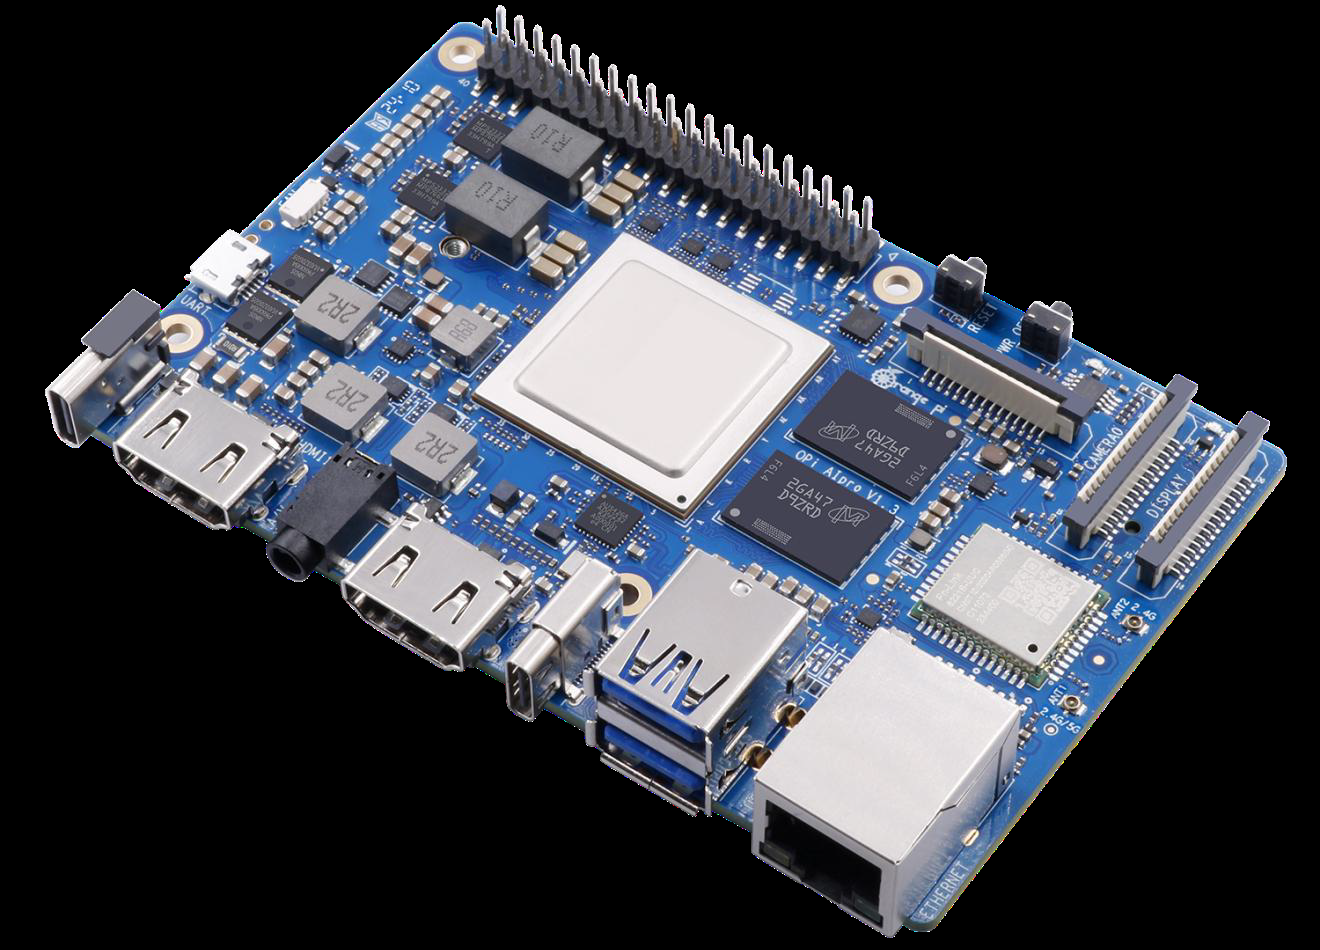
\includegraphics{img0/aipro.png}

\hypertarget{ux5f00ux53d1ux677fux8be6ux7ec6ux89c6ux56fe}{%
\subsection{开发板详细视图}\label{ux5f00ux53d1ux677fux8be6ux7ec6ux89c6ux56fe}}

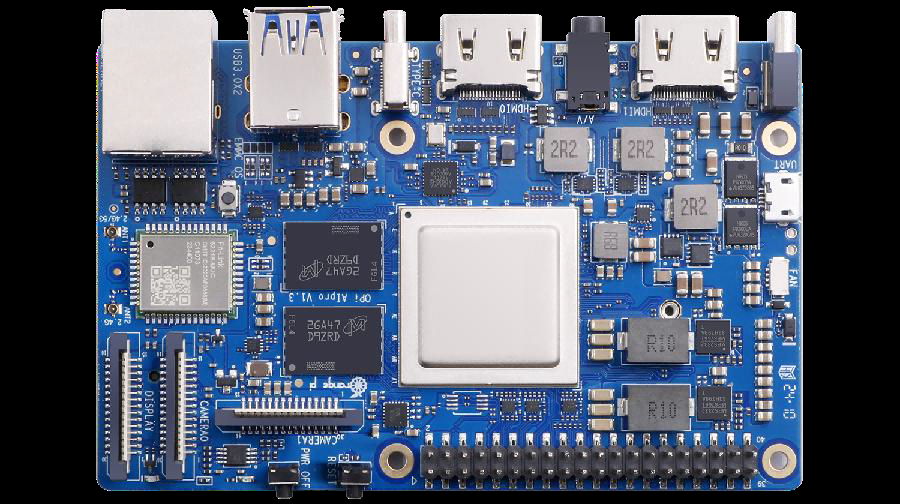
\includegraphics{img0/4.png} 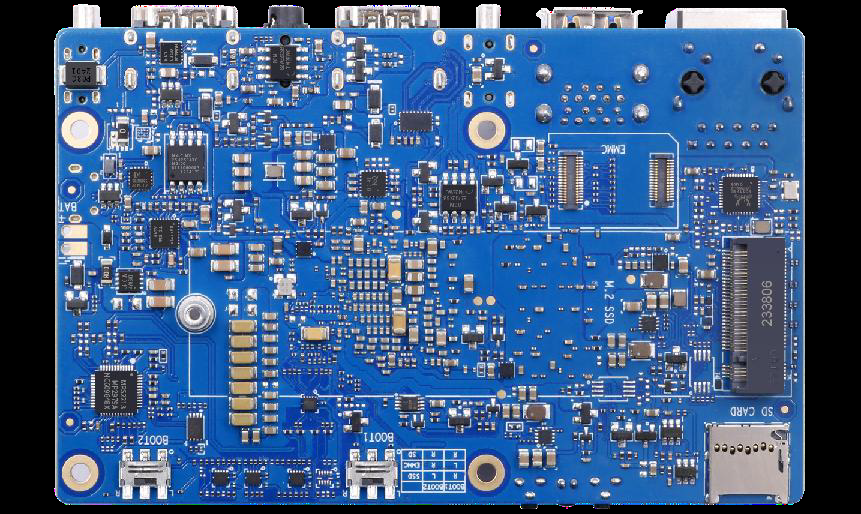
\includegraphics{img0/5.png}
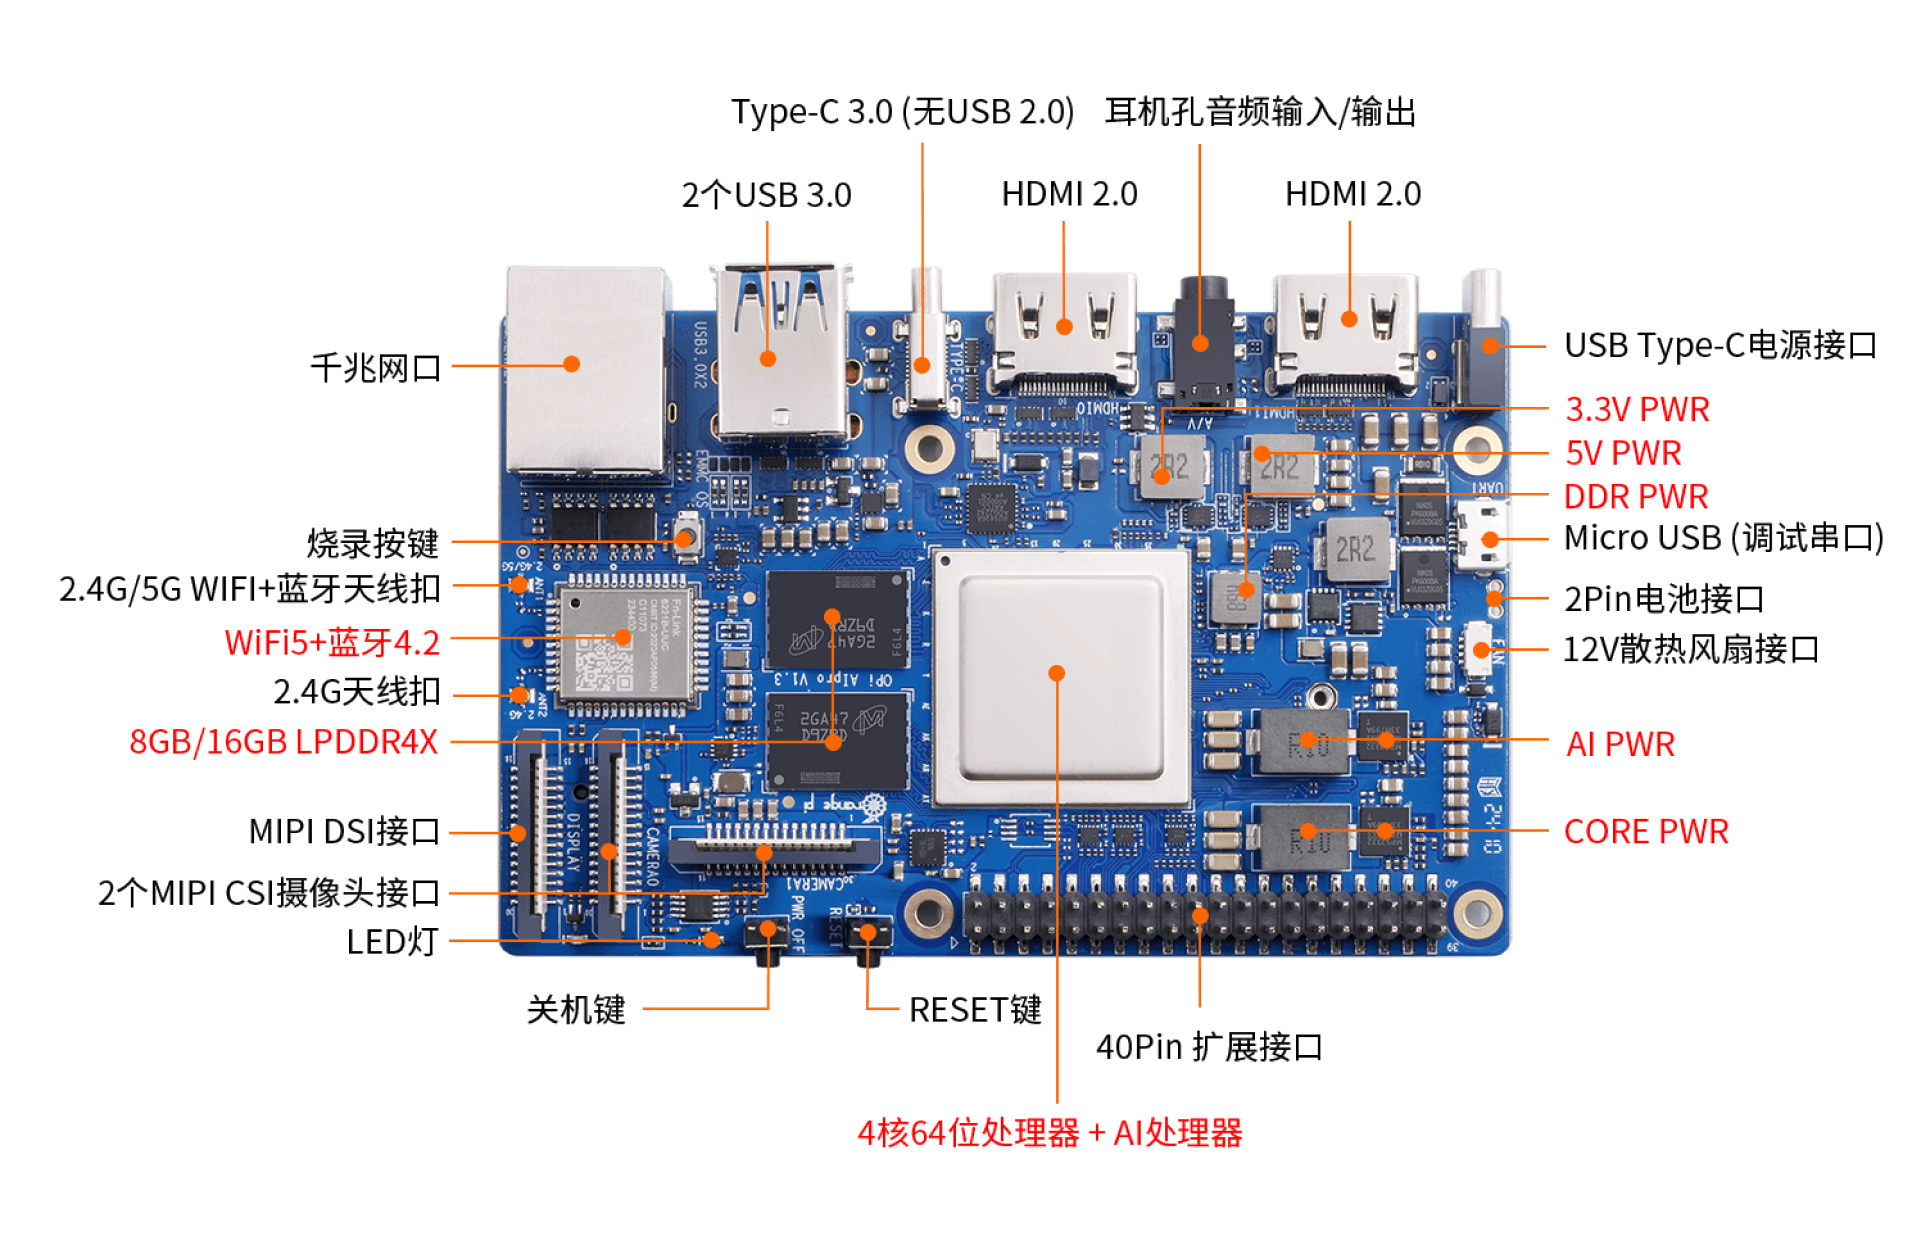
\includegraphics{img0/1.png} 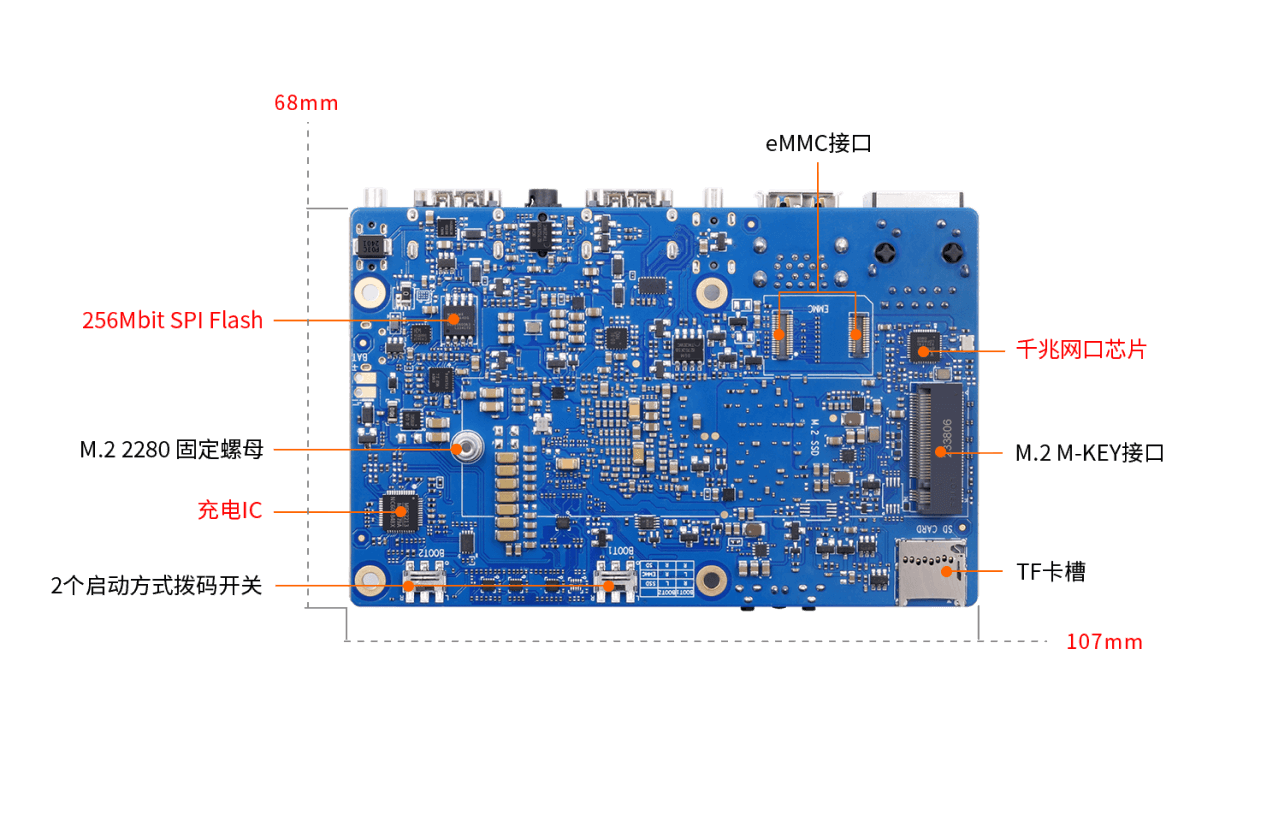
\includegraphics{img0/2.png}
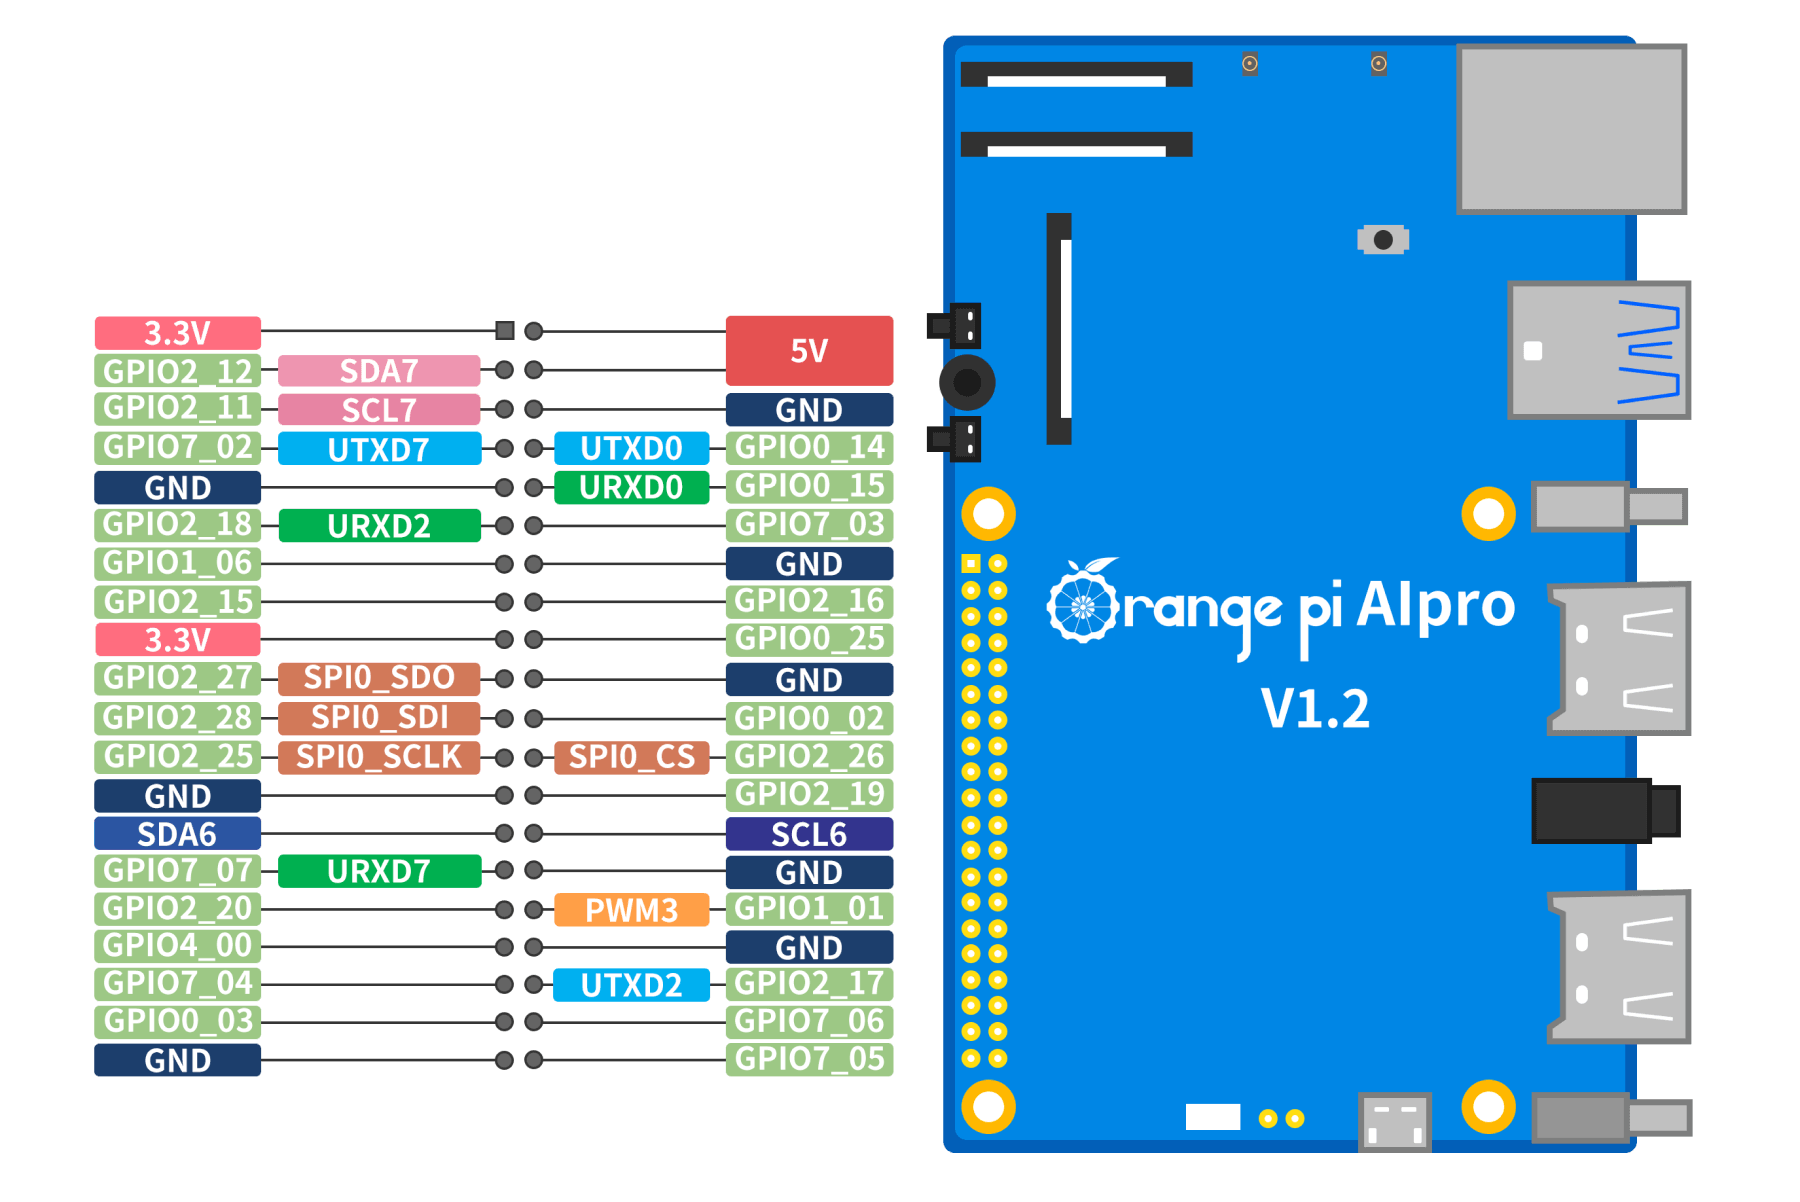
\includegraphics{img0/3.png}

\hypertarget{ux5f00ux53d1ux677fux786cux4ef6ux89c4ux683c}{%
\subsection{开发板硬件规格}\label{ux5f00ux53d1ux677fux786cux4ef6ux89c4ux683c}}

\begin{center}\rule{0.5\linewidth}{0.5pt}\end{center}

\hypertarget{ux6240ux9700ux914dux4ef6}{%
\subsection{所需配件}\label{ux6240ux9700ux914dux4ef6}}

\begin{enumerate}
\def\labelenumi{\arabic{enumi}.}
\item
  TF卡
  容量最小为32GB,速率为Class10级以上的闪迪品牌的TF卡,如下图所示。建议使用64G及以上的TF卡,以避免在开发过程中出现磁盘空间不足的问题。
  
\includegraphics{img1/tf.jpg}
\item
  TF卡读卡器
  用于读写TF卡,刷写系统,建议选择速率为USB3.0以上的,减少系统刷写的等待时间。
  
\includegraphics{img1/reader.jpg}
\item
  HDMI线或HDMI转mini-HDMI线
  主要取决于显示器的接口类型该开发板的视频输出接口为标准HDMI接口。
  
\includegraphics{img1/hdmi.jpg} 
\includegraphics{img1/minihdmi.jpg}
\item
  电源 该开发板的电源输入为PD
  20V,需要搭配支持PD协议20V挡位的65W电源适配器。
  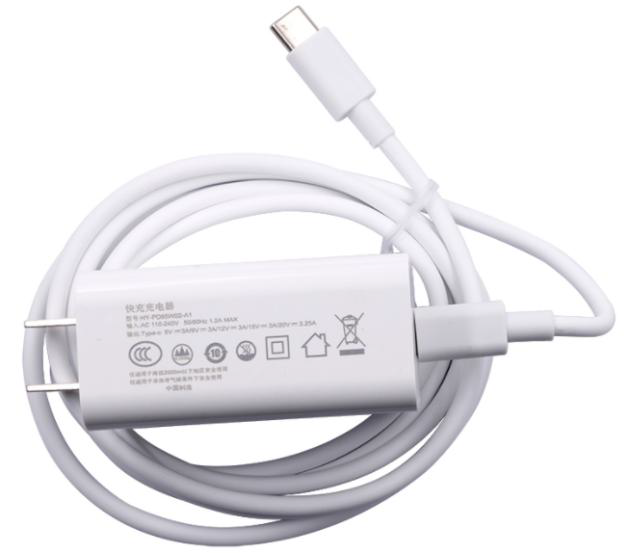
\includegraphics{img1/power.png}
\item
  USB接口的鼠标以及键盘 在无远程访问的条件下对开发板进行本地调试。
  
\includegraphics{img1/mouse.png}
\item
  金属配套外壳 用于保护开发板硬件。 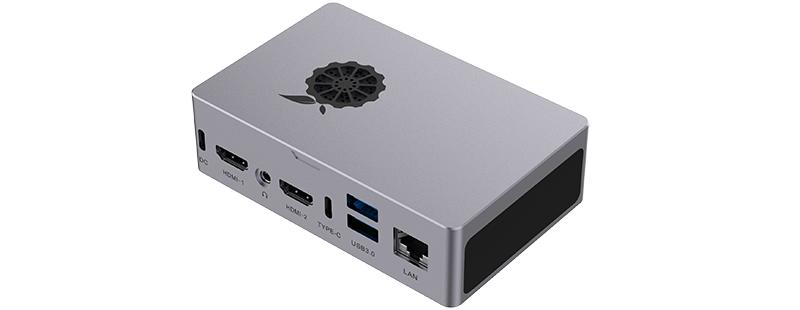
\includegraphics{img1/cover.png}
\item
  12V散热风扇以及散热鳍块
  开发板的风扇接口为2pin,输出电压为12v,支持PWM调速。由于该开发板的CPU发热较大,强烈建议安装主动扇热设备。
  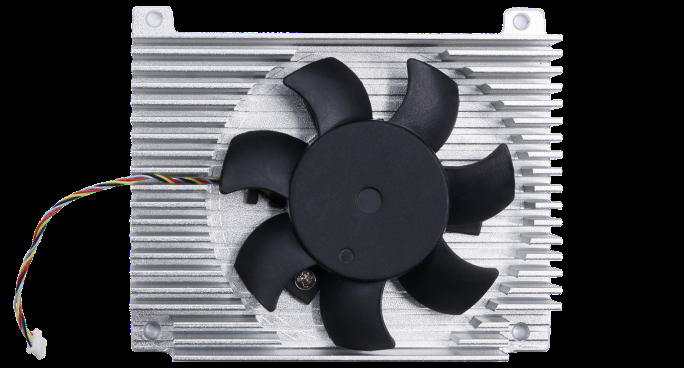
\includegraphics{img1/fan.png}
\item
  Type-C转USB 3.0转接线(可选) OrangePi
  AIPro开发板具有一个Type-C接口,协议为USB3.0(不支持USB
  2.0),可外接支持USB3.0以上协议的外置设备。
  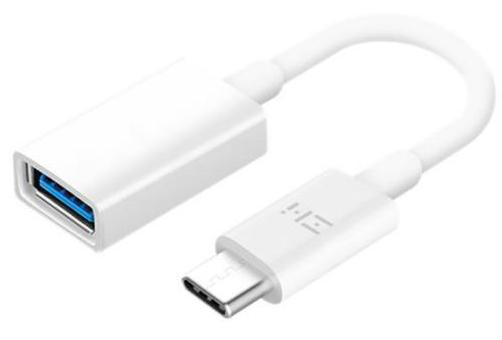
\includegraphics{img1/otg.png}
\item
  M.2接口 2280规格的PCIe Nvme SSD(可选)
  开发板的背部设计有M.2接口,可外接一个M.2的SSD作为开发板的系统盘或者存储。
  
\includegraphics{img1/nvme.png}
\item
  M.2接口 2280规格的Sata Ngff SSD(可选)
  同样,开发板的M.2接口不仅支持PCIe协议,也支持Sata协议,因此也可以使用Sata协议的SSD。
  
\includegraphics{img1/ngff.png}
\item
  香橙派的eMMC模块(可选)
  eMMC(嵌入式多媒体卡)是一种集成了闪存和控制器的低成本存储解决方案,主要用于智能手机、平板电脑和低端笔记本电脑等消费电子产品。其读写速度适中(100-400MB/s),比传统机械硬盘快但不及固态硬盘(SSD),具有体积小、功耗低和易于集成的特点。开发板支持使用eMMC模块作为存储,但需要额外购置eMMC模块。
  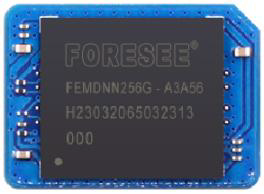
\includegraphics{img1/emmc1.png} 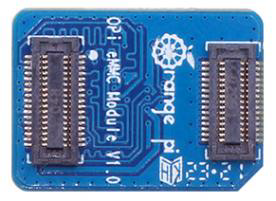
\includegraphics{img1/emmc2.png}
\item
  USB摄像头模块(可选) 可用于图像识别、视频通话等多方面用途。
  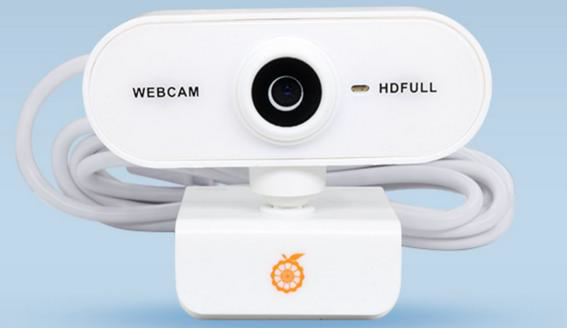
\includegraphics{img1/camera.png}
\item
  网线(可选)
  开发板自带有wifi模块可用于连接wifi,若需要更稳定的网络连接,建议使用网线连接。
  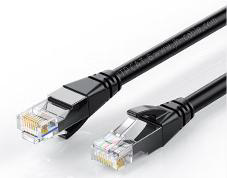
\includegraphics{img1/cable.png}
\item
  树莓派IMX219型号摄像头(MIPI-CSI)(可选)
  开发板带有两个MIPI-CSI接口,可以兼容树莓派的MIPI摄像头,无需占用USB接口。
  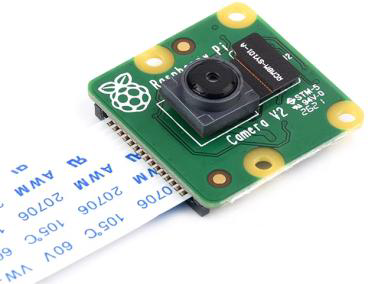
\includegraphics{img1/csi.png}
\item
  树莓派5寸MIPI LCD显示屏(可选)
  开发板带有一个MIPI-DSI显示输出接口,可以直接驱动MIPI的显示屏,而无需外接显示器。
  
\includegraphics{img1/dsi.png}
\item
  Micro USB数据线(可选) 开发板自带了CH343P芯片,将UART转发为Micro
  USB接口,若需要使用串口对开发板进行调试,则需要使用Micro USB数据线。
  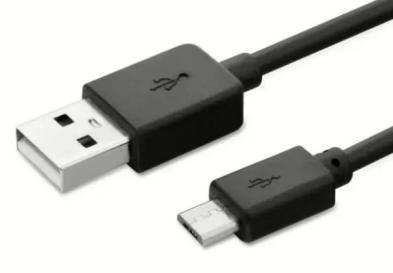
\includegraphics{img1/microusb.png}
\end{enumerate}

\hypertarget{ux4e0bux8f7dux5f00ux53d1ux677fux7684ux7cfbux7edfux955cux50cf}{%
\subsection{下载开发板的系统镜像}\label{ux4e0bux8f7dux5f00ux53d1ux677fux7684ux7cfbux7edfux955cux50cf}}

作为华为生态中重要的一员,开发板不仅支持Ubuntu系统,也支持openEuler系统,但由于开发板自身并无存储,我们在使用开发板的过程中需要使用电脑对TF卡进行系统的刷写,建议使用安装有Windows11
或 Ubuntu22.04以上版本的PC。

首先,打开香橙派官网的\href{http://www.orangepi.cn/html/hardWare/computerAndMicrocontrollers/service-and-support/Orange-Pi-AIpro.html}{技术支持界面}。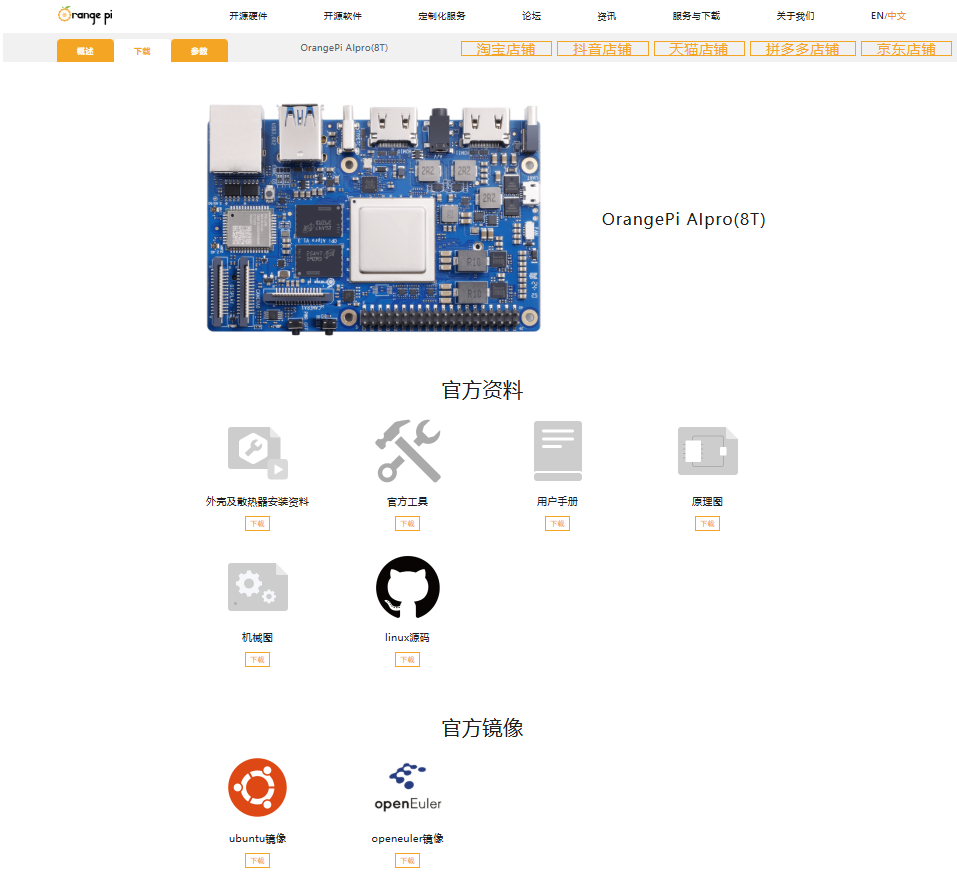
\includegraphics{img1/技术支持.png}

向下滑动网页,找到官方镜像部分,分为Ubuntu和openEuler两个部分,两个系统都是官方为我们编译完成的,且预装了部分昇腾NPU的应用环境以及软件,非常方便新手用户上手使用。

\includegraphics{img1/官方镜像.png}

\hypertarget{ubuntu}{%
\subsubsection{Ubuntu}\label{ubuntu}}

\begin{enumerate}
\def\labelenumi{\arabic{enumi}.}
\tightlist
\item
  点击下载
\includegraphics{img1/download_ubuntu.png}
\item
  复制提取码并跳转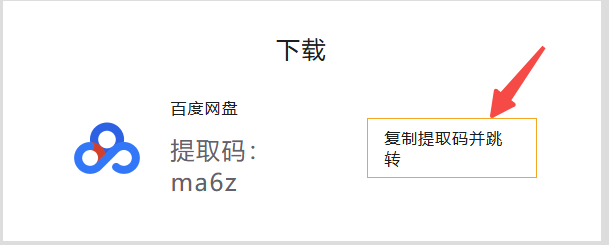
\includegraphics{img1/copyandjump.png}
\item
  打开百度网盘的链接后有一个命名为Ubuntu的文件夹,点开该文件夹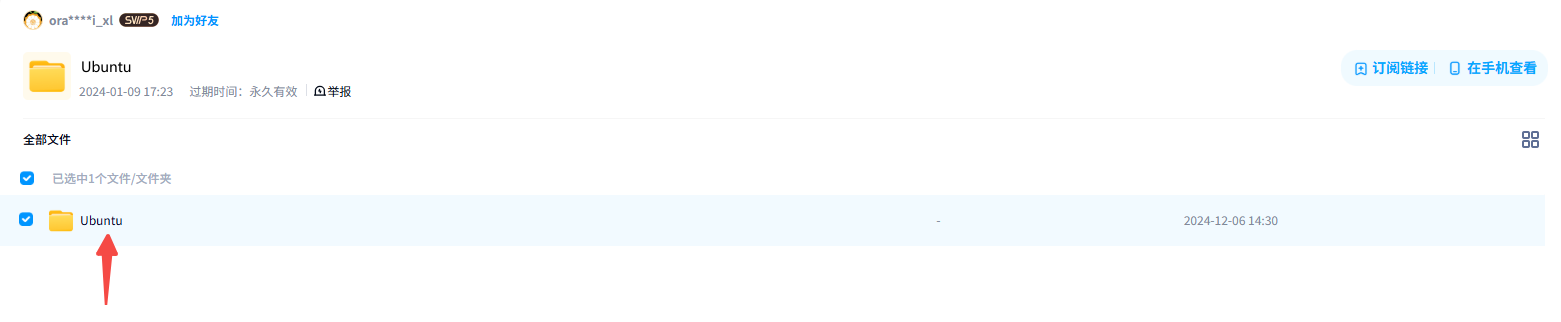
\includegraphics{img1/folder.png}
\item
  文件夹中,后缀为.xz的文件是镜像压缩包文件,.sha文件是压缩包的md5校验码文件,用于校验镜像包文件是否完整。
\item
  文件夹中的镜像有两种,一种文件名带有Desktop的,是带有GUI图形化界面的,另一种文件名带有minimal的,是不具有图形化界面的,只有命令行界面。建议新学习的用户使用带有desktop的镜像。
  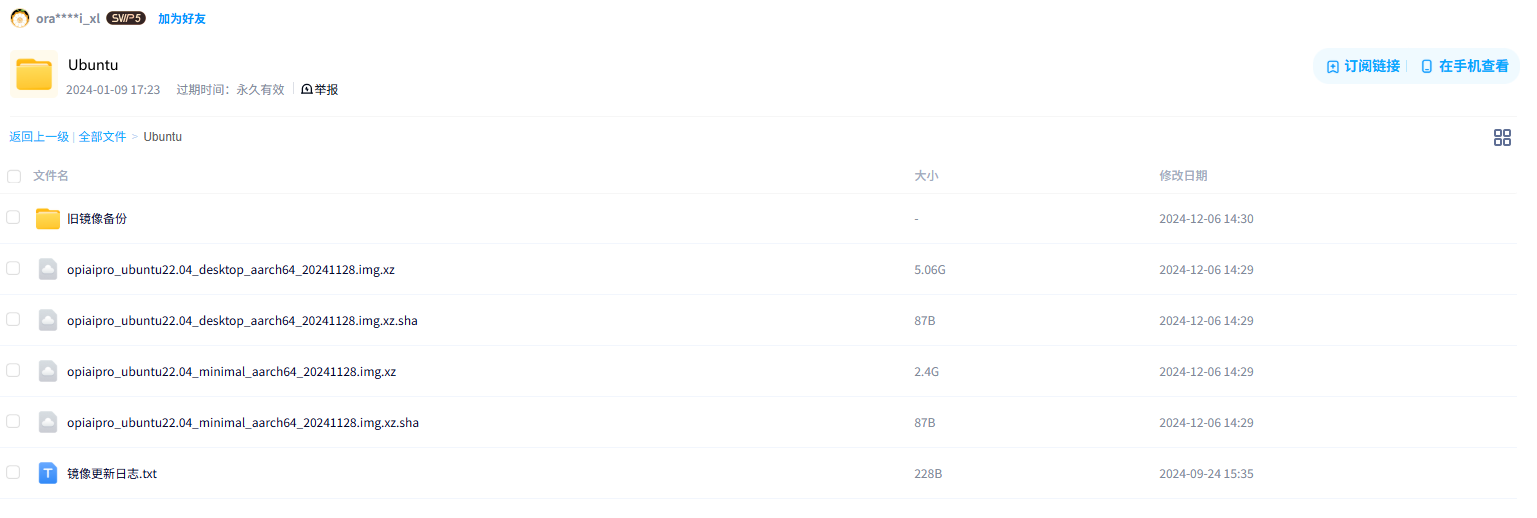
\includegraphics{img1/chooseubuntu.png}
\item
  下载后先校验压缩包是否完整,后解压压缩包
\end{enumerate}

\hypertarget{openeuler}{%
\subsubsection{openEuler}\label{openeuler}}

\begin{enumerate}
\def\labelenumi{\arabic{enumi}.}
\tightlist
\item
  点击下载
\includegraphics{img1/download_openeuler.png}
\item
  复制提取码并跳转
\includegraphics{img1/cpjp.png}
\item
  打开百度网盘的链接后有一个命名为OpenEuler的文件夹,点开该文件夹
\includegraphics{img1/folderr.png}
\item
  文件夹中,后缀为.xz的文件是镜像压缩包文件,.sha文件是压缩包的md5校验码文件,用于校验镜像包文件是否完整。
\item
  文件夹中的镜像只有一种,即具有GUI图形化界面的openEuler系统。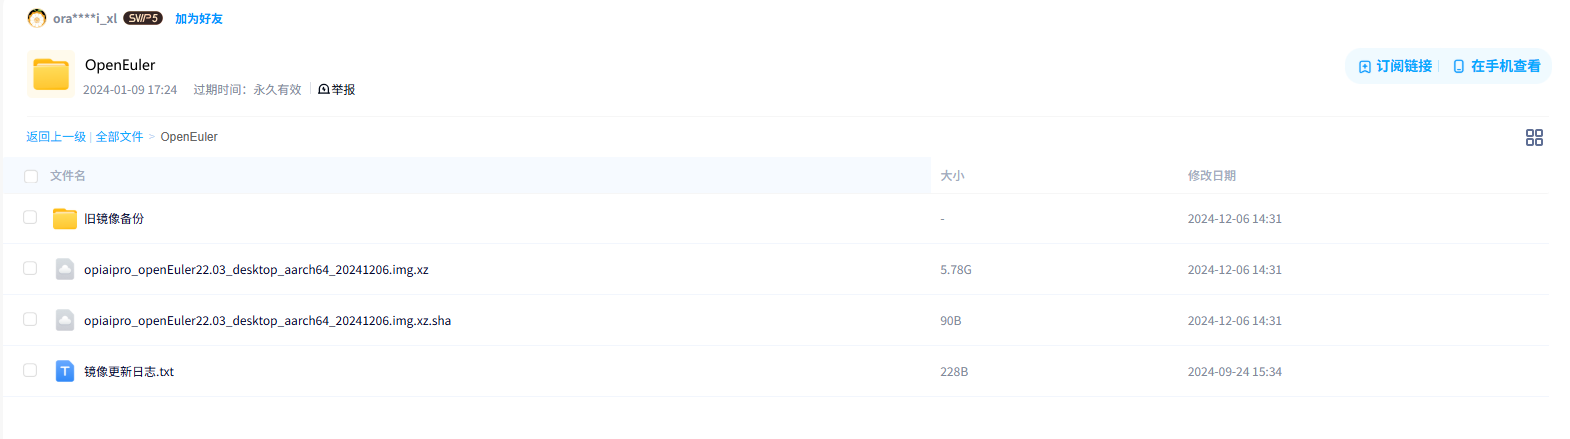
\includegraphics{img1/chooseeuler.png}
\item
  下载后先校验压缩包是否完整,后解压压缩包
\end{enumerate}

\hypertarget{ux4f7fux7528md5ux6821ux9a8cux4e0bux8f7dux7684ux6587ux4ef6}{%
\subsubsection{使用md5校验下载的文件}\label{ux4f7fux7528md5ux6821ux9a8cux4e0bux8f7dux7684ux6587ux4ef6}}

在Windows系统下,可以使用\texttt{certutil\ -hashfile\ \textless{}filename\textgreater{}\ md5};在Ubuntu系统下,可以使用\texttt{md5sum\ \textless{}filename\textgreater{}};在MacOS系统下,可以使用\texttt{md5\ \textless{}filename\textgreater{}}进行计算,此处以Windows系统为例:在文件夹按住Shift键并单击鼠标右键,选择``在终端(Powershell/命令提示符)中打开''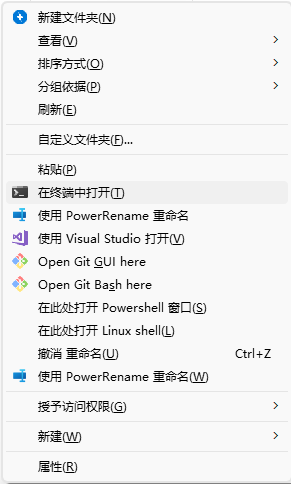
\includegraphics{img1/shell.png},然后在打开的窗口中输入\texttt{certutil\ -hashfile\ opiaipro\_ubuntu22.04\_desktop\_aarch64\_20241128.img.xz\ md5}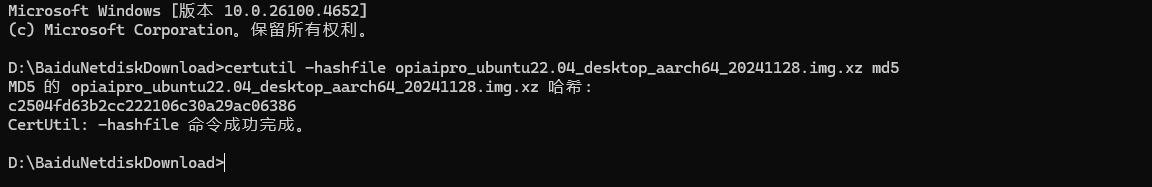
\includegraphics{img1/md5.png},将得到的md5值与\texttt{opiaipro\_ubuntu22.04\_desktop\_aarch64\_20241128.img.xz.sha}文件进行对比,若一致可进行下一步操作,否则需要重新下载。

\hypertarget{ux5237ux5199ux7cfbux7edfux5230tfux5361}{%
\subsection{刷写系统到TF卡}\label{ux5237ux5199ux7cfbux7edfux5230tfux5361}}

\hypertarget{ux4e0bux8f7dux5e76ux5b89ux88c5ux5fc5ux8981ux7684ux5de5ux5177}{%
\subsubsection{下载并安装必要的工具}\label{ux4e0bux8f7dux5e76ux5b89ux88c5ux5fc5ux8981ux7684ux5de5ux5177}}

\begin{quote}
下载链接:\href{http://www.orangepi.cn/html/hardWare/computerAndMicrocontrollers/service-and-support/Orange-Pi-AIpro.html}{官网}
\href{https://pan.baidu.com/s/1Jho73pw91r5GJD2KijY45Q?pwd=3xuz\#list/path=\%2F}{百度网盘}
1. SD Card Formatter
这个是TF卡的快速格式化工具,在每次需要刷写系统之前,都必须先对TF卡进行格式化操作,若不格式化在后续的刷写系统过程中有较大概率出错。
2. balenaEther 这个是系统镜像的刷写工具,用于刷写img镜像文件进入TF卡。
\end{quote}

\hypertarget{ux683cux5f0fux5316tfux5361}{%
\subsubsection{格式化TF卡}\label{ux683cux5f0fux5316tfux5361}}

\begin{enumerate}
\def\labelenumi{\arabic{enumi}.}
\tightlist
\item
  将TF卡插入读卡器中,并将读卡器插入电脑
\item
  打开SD Card Formatter软件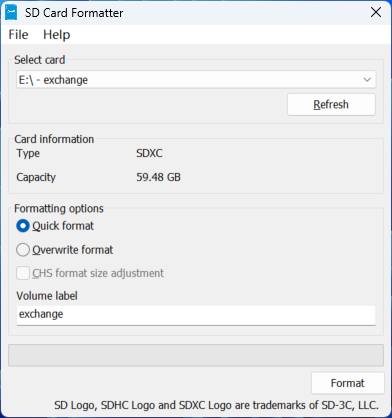
\includegraphics{img1/SDFmt.png}
\item
  点击右下角Format按键,格式化TF卡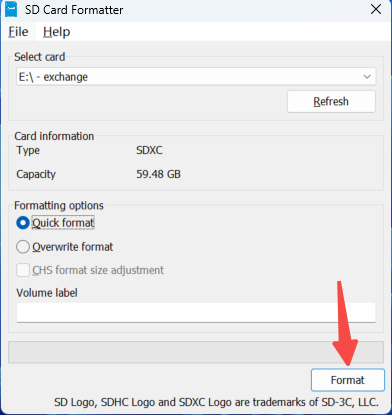
\includegraphics{img1/fmt.png}
  \textgreater{}
  警告内容是关于格式化操作会清除TF卡上原有的所有数据,此处选是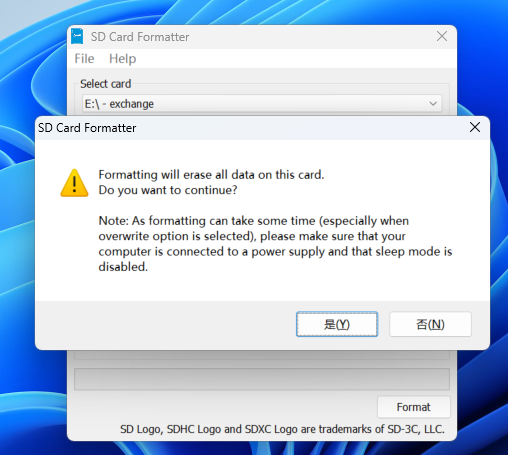
\includegraphics{img1/warning.png}
\item
  等待软件格式化完成,并点击确定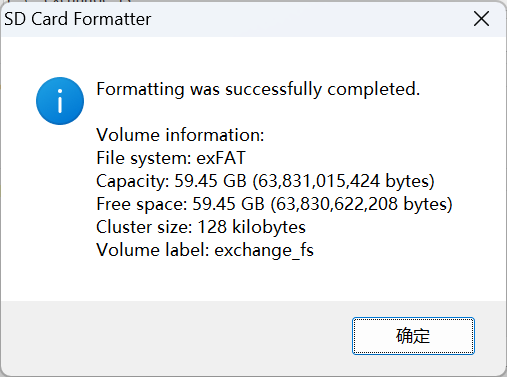
\includegraphics{img1/fmtfin.png}
\end{enumerate}

\hypertarget{ux5237ux5199ux7cfbux7edfux5230tfux5361ux4ee5ubuntuux4e3aux4f8b}{%
\subsubsection{刷写系统到TF卡(以Ubuntu为例)}\label{ux5237ux5199ux7cfbux7edfux5230tfux5361ux4ee5ubuntuux4e3aux4f8b}}

\begin{quote}
此处以Ubuntu为例 1.
打开balenaEther,选择``从文件烧录''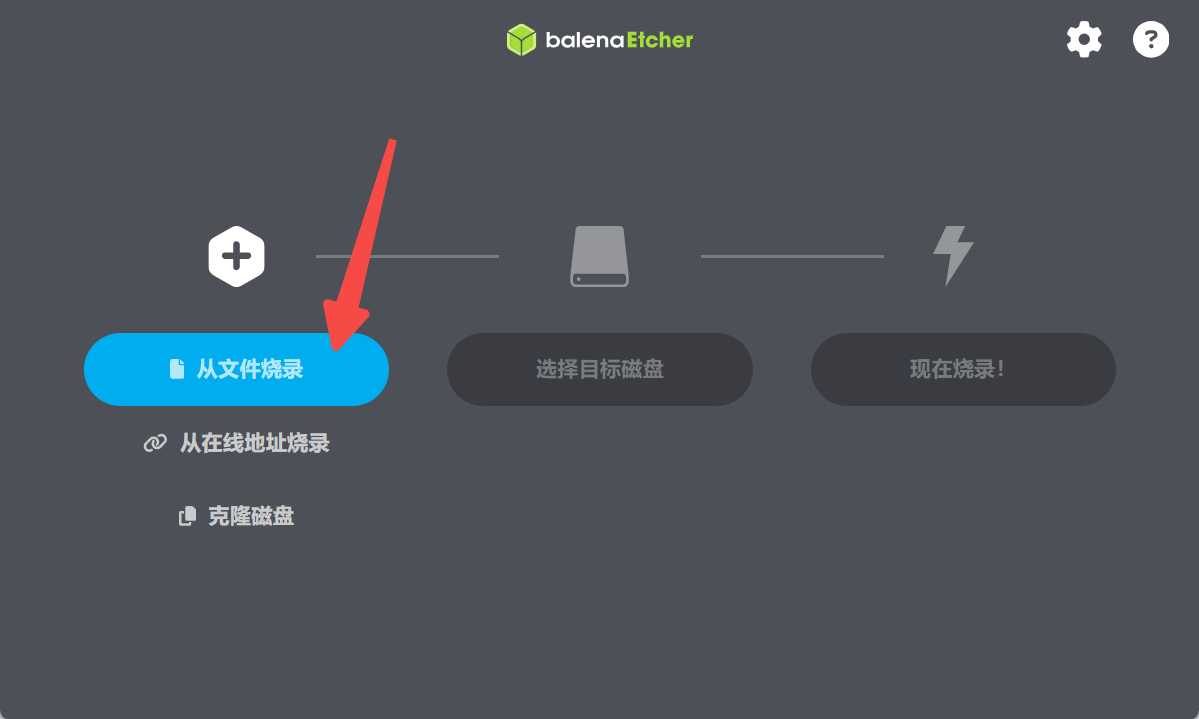
\includegraphics{img1/ether1.png} 2.
选择好要烧录的镜像文件(\textbf{.img}格式),再选择目标磁盘为TF卡对应的位置,如图中名称为``SDXC
Card''的位置,选中并选择``选定1''。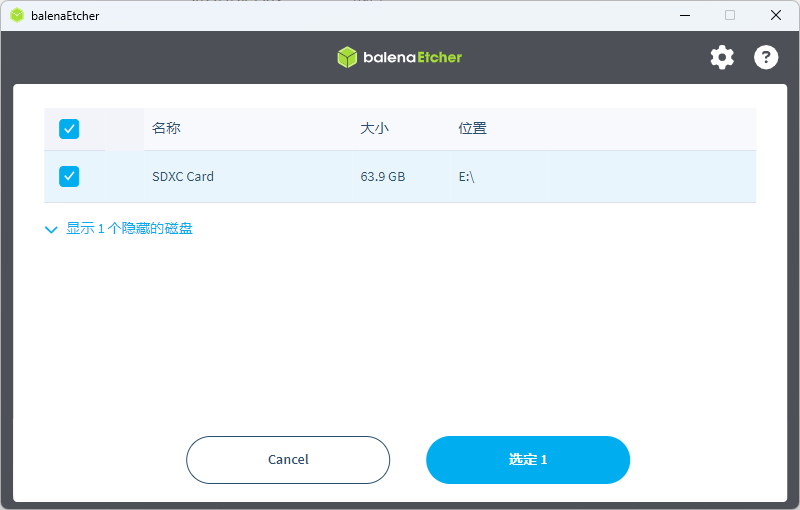
\includegraphics{img1/chooseether.png}
3. 点击``现在烧录!'',耐心等待烧录完成。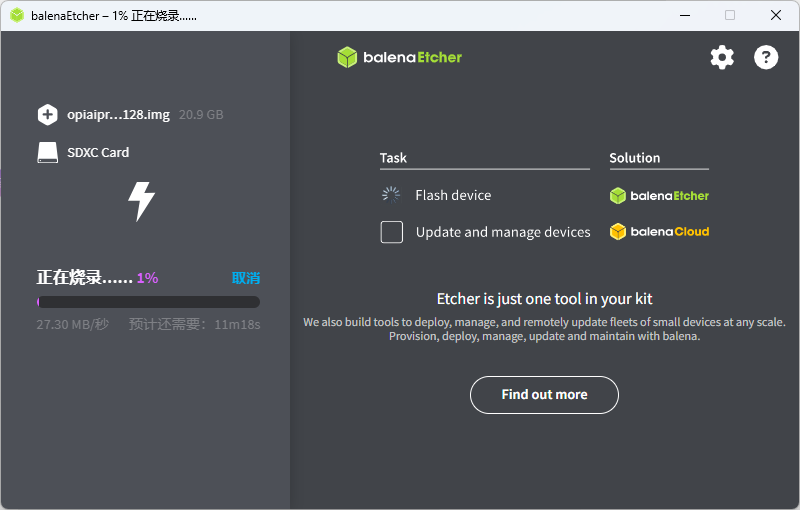
\includegraphics{img1/dd.png}
4. 烧录完成后进入校验过程,也请耐心等待。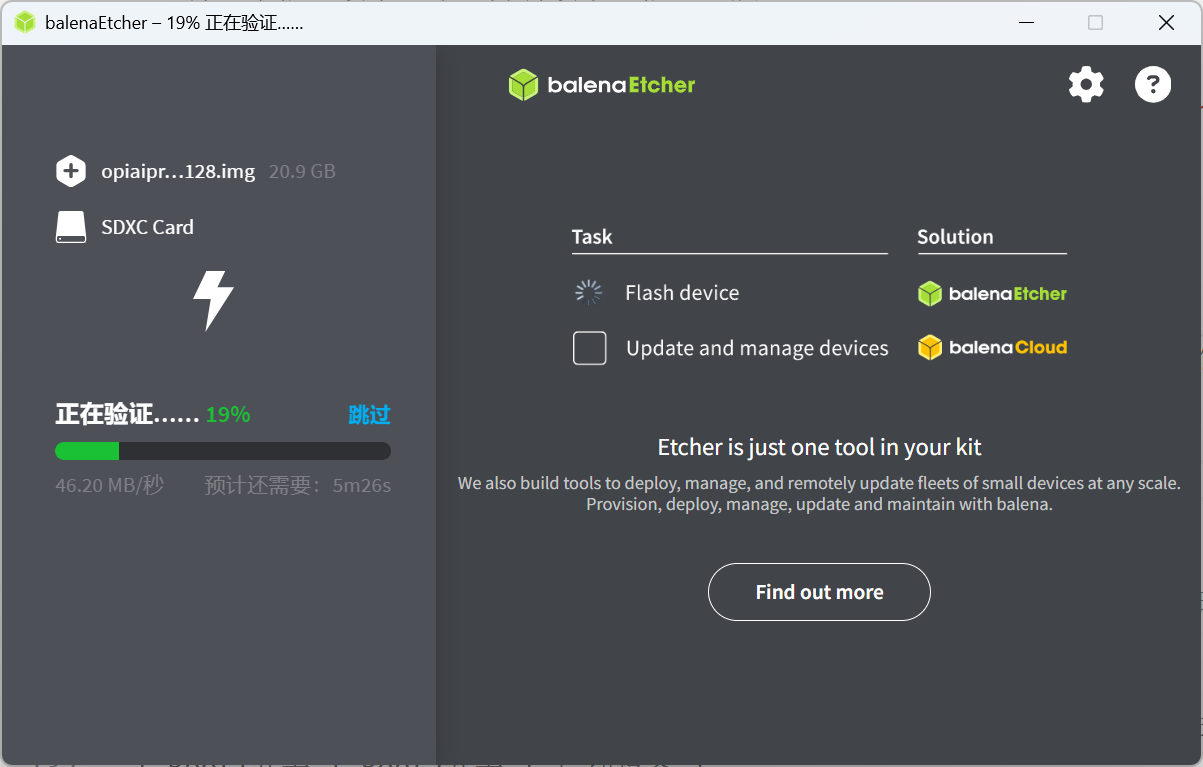
\includegraphics{img1/val.png}
5.
烧录完成后即可关闭程序,并安全弹出TF卡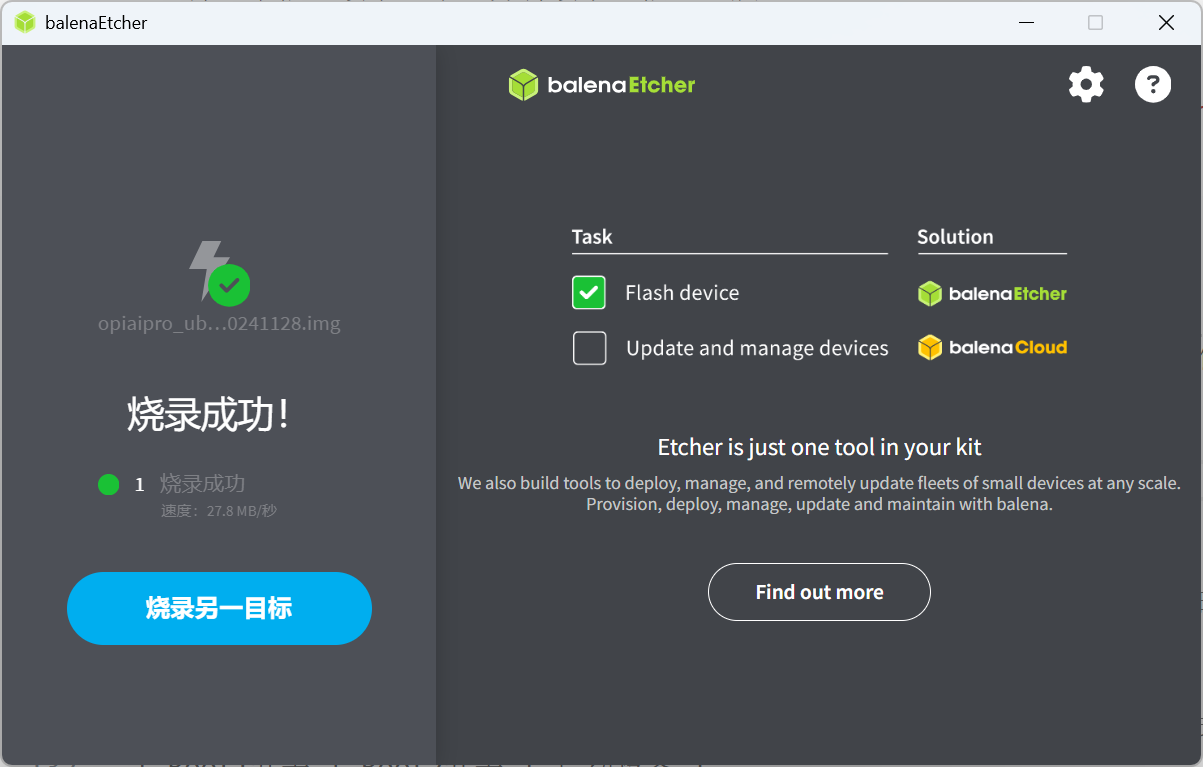
\includegraphics{img1/finish.png}
\end{quote}

\hypertarget{ux5237ux5199ux7cfbux7edfux5230emmc}{%
\subsubsection{刷写系统到eMMC}\label{ux5237ux5199ux7cfbux7edfux5230emmc}}

由于板上并不自带有eMMC模块,若要想使用需要额外购买香橙派的eMMC模块,此处暂时不列入参考,若需使用,请查阅香橙派的用户手册。

\hypertarget{ux5237ux5199ux7cfbux7edfux5230ssd}{%
\subsubsection{刷写系统到SSD}\label{ux5237ux5199ux7cfbux7edfux5230ssd}}

开发板带有M.2接口,可以使用SSD作为启动设备。但SSD需要自行准备,且根据香橙派

\hypertarget{ux8c03ux6574ux8bbeux5907ux542fux52a8ux65b9ux5f0fux7684ux62e8ux7801ux5f00ux5173}{%
\subsubsection{调整设备启动方式的拨码开关}\label{ux8c03ux6574ux8bbeux5907ux542fux52a8ux65b9ux5f0fux7684ux62e8ux7801ux5f00ux5173}}

开发板支持多种启动方式,包括TF卡、eMMC以及M.2
SSD,当这些存储设备都同时存在时,需要让开发板选定一个存储设备作为启动来源。
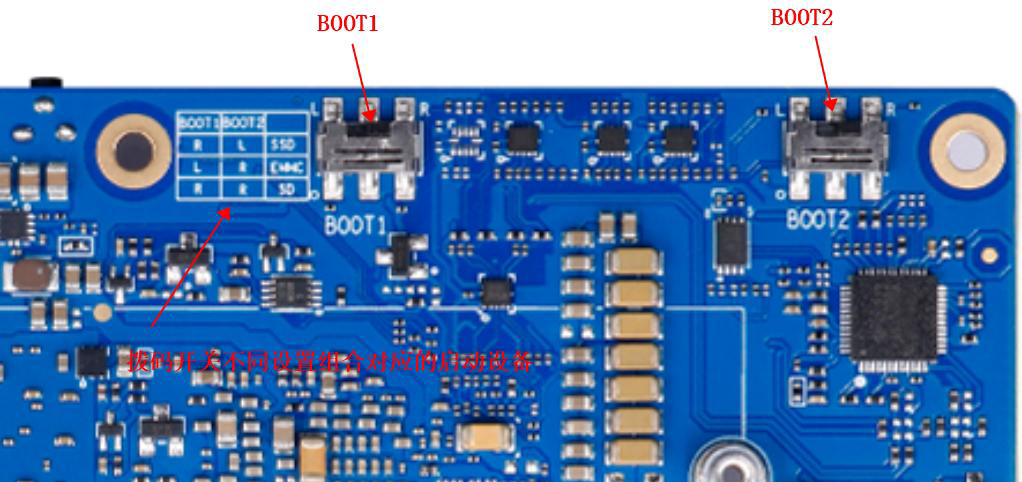
\includegraphics{img1/bootswitch.png}
两个开关都有左、右两种状态,因此共有4种状态,但是目前开发板仅使用3种模式,对应的参数表如下:
\textbar{} Boot1开关 \textbar{} Boot2开关 \textbar{} 启动设备 \textbar{}
\textbar{} :------: \textbar{} :------: \textbar{} :------: \textbar{}
\textbar{} 左 \textbar{} 左 \textbar{} 未使用 \textbar{} \textbar{} 右
\textbar{} 右 \textbar{} TF卡 \textbar{} \textbar{} 左 \textbar{} 右
\textbar{} eMMC \textbar{} \textbar{} 右 \textbar{} 左 \textbar{} M.2
SSD (Nvme或Ngff)\textbar{}
切换拨码开关后,必须要将开发板完全断电再重新上电才能使新的启动配置生效,使用RESET按键重启则不会使新的启动配置生效。

\hypertarget{ux542fux52a8ux5f00ux53d1ux677fubuntu}{%
\subsection{启动开发板(Ubuntu)}\label{ux542fux52a8ux5f00ux53d1ux677fubuntu}}

\begin{itemize}
\tightlist
\item
  图形化界面
\end{itemize}

\begin{enumerate}
\def\labelenumi{\arabic{enumi}.}
\tightlist
\item
  将系统刷写完成的TF卡从读卡器中取出,插入开发板的TF卡插槽中,并确保两个启动开关的位置均在右边,接入HDMI数据线到靠近USB3.0接口的HDMI0接口,然后将Type-C电源线插入开发板最边缘的TYPE-C供电口,等待风扇的声音变小以及屏幕出现系统登录界面。
  
\includegraphics{img1/beforelogin.png}
\item
  进入登录界面后,将键盘接入开发板的USB接口中,默认的登录用户名是\texttt{HwHiAiUser},输入该账户的密码\texttt{Mind@123},登录进入系统。
  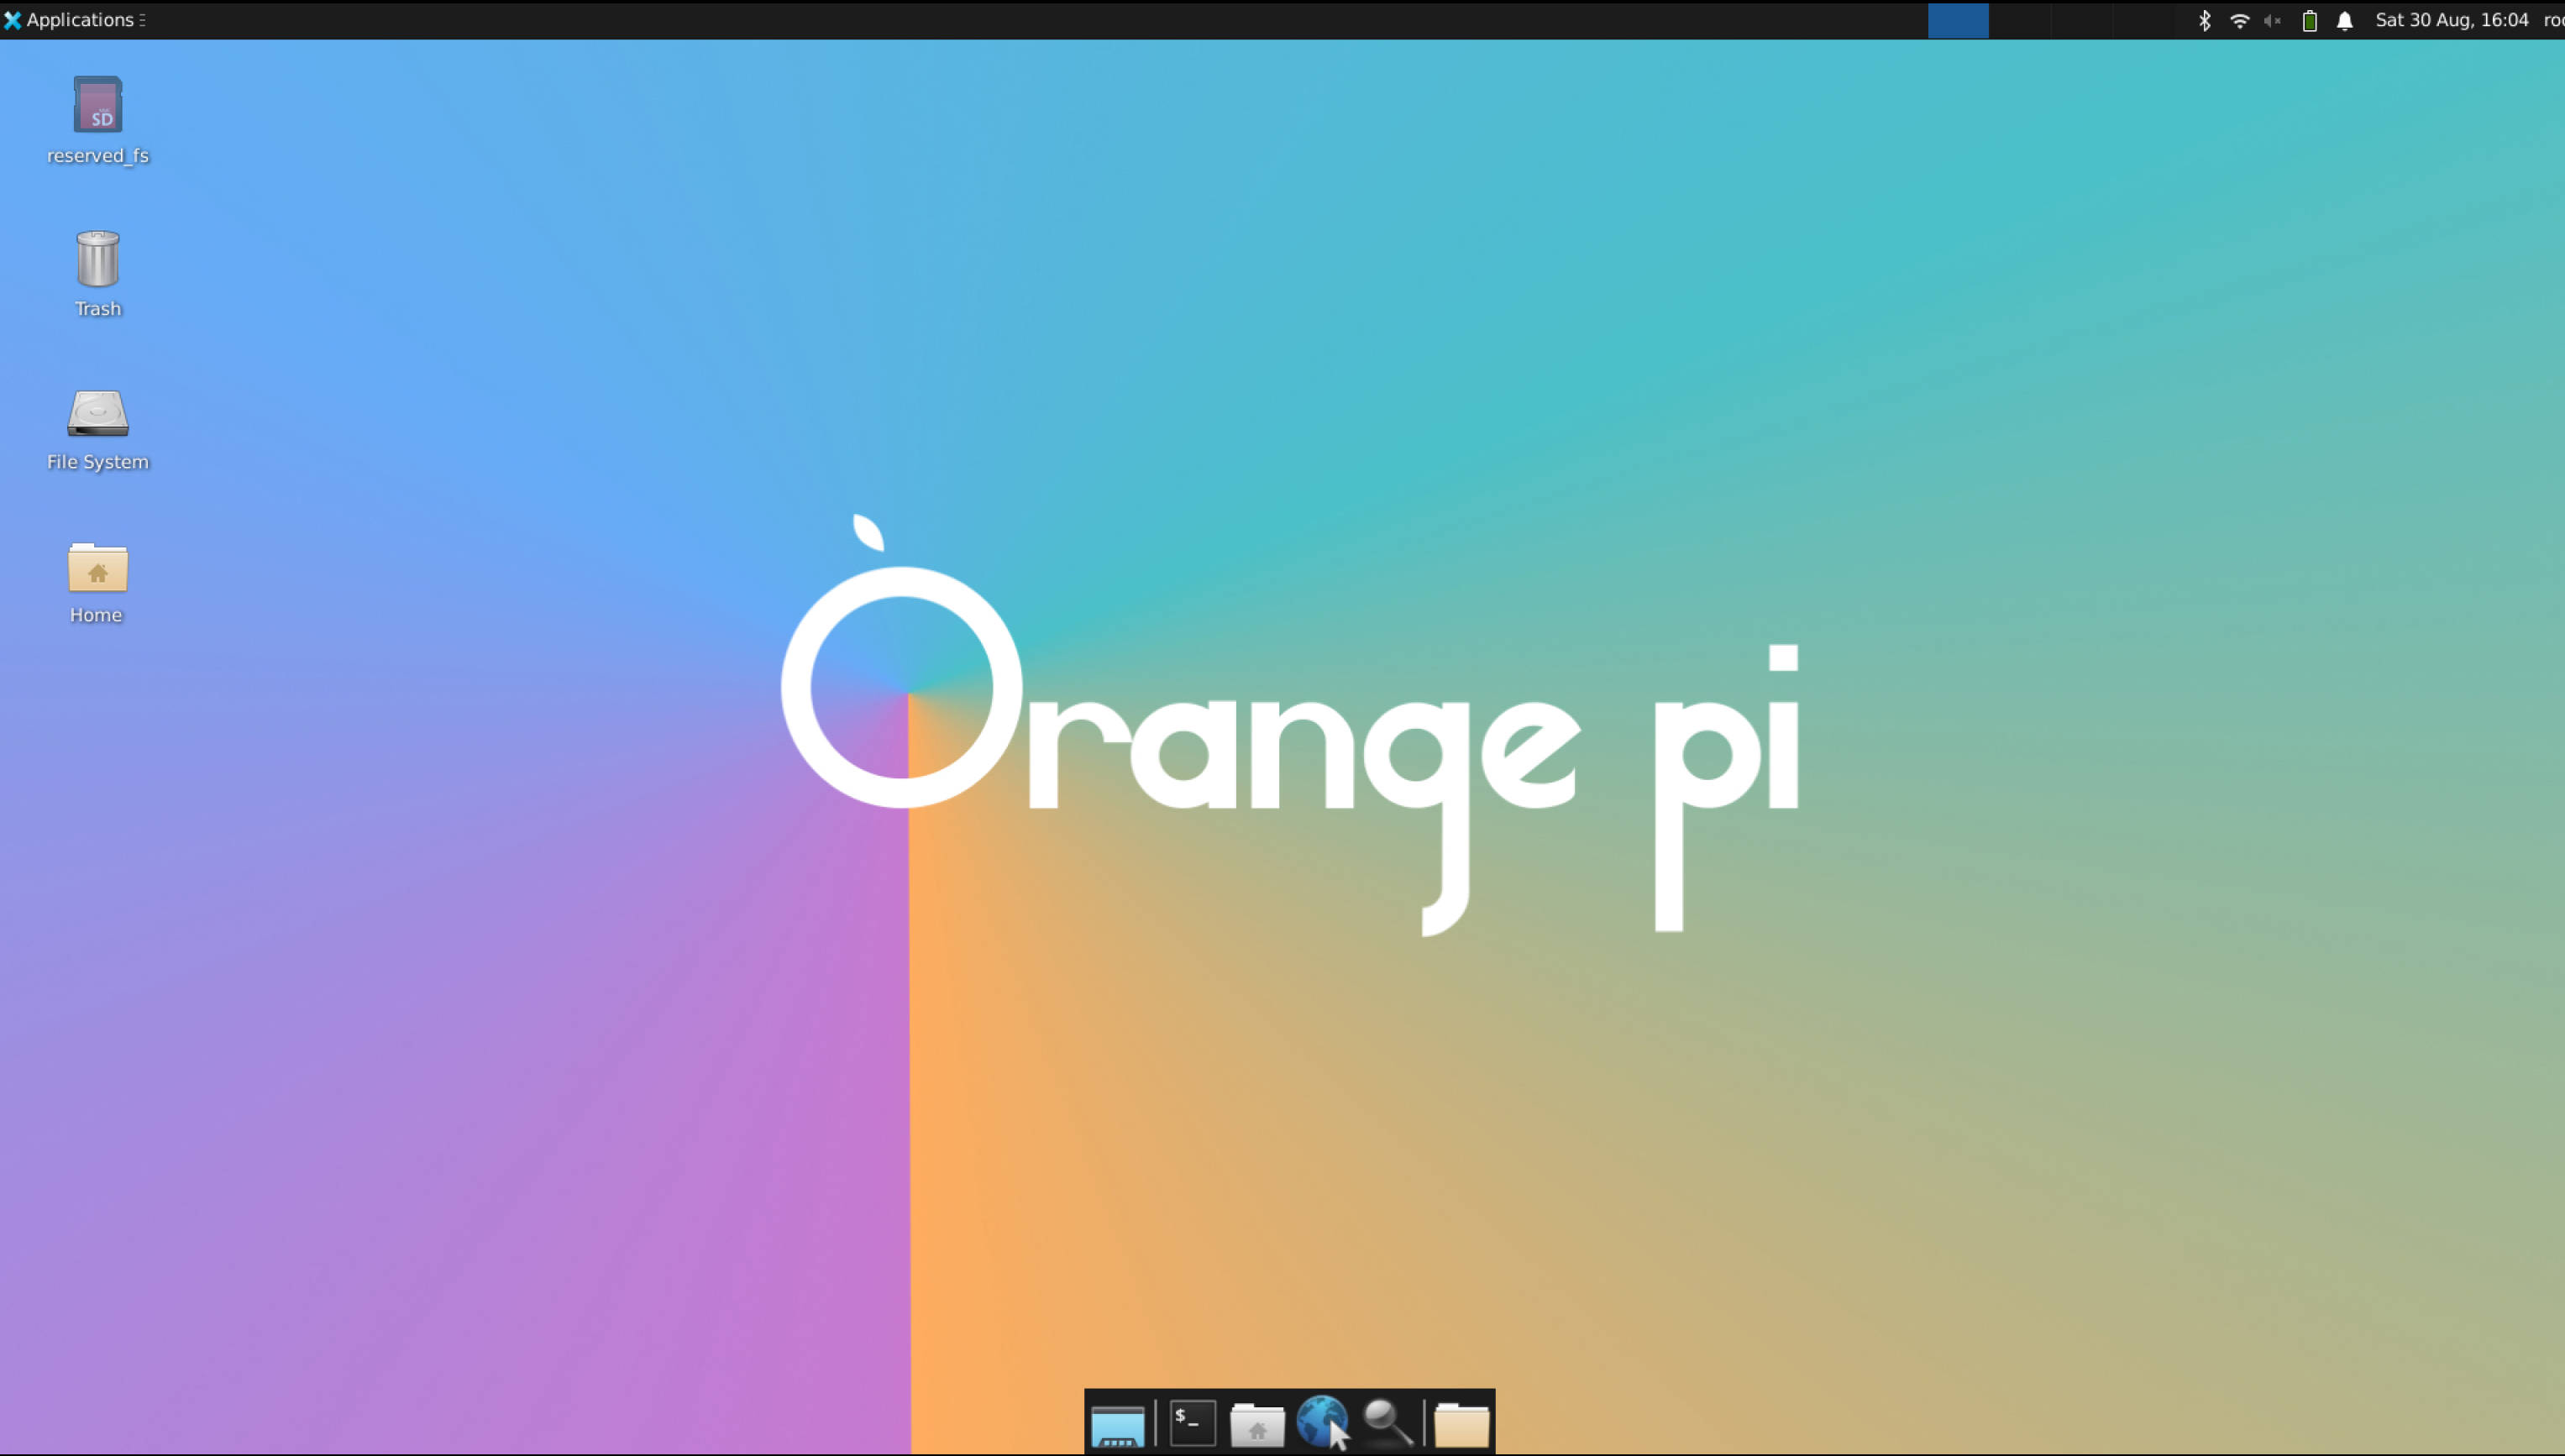
\includegraphics{img1/logingui.png} 默认账户表格: \textbar{} 用户名
  \textbar{} 密码 \textbar{} \textbar{} :---: \textbar{} :--: \textbar{}
  \textbar{} root \textbar{} Mind@123 \textbar{} \textbar{} HwHiAiUser
  \textbar{} Mind@123 \textbar{}
\end{enumerate}

\begin{itemize}
\tightlist
\item
  串口界面
\end{itemize}

\begin{enumerate}
\def\labelenumi{\arabic{enumi}.}
\tightlist
\item
  使用USB2TTL模块,与开发板的GPIO口进行连线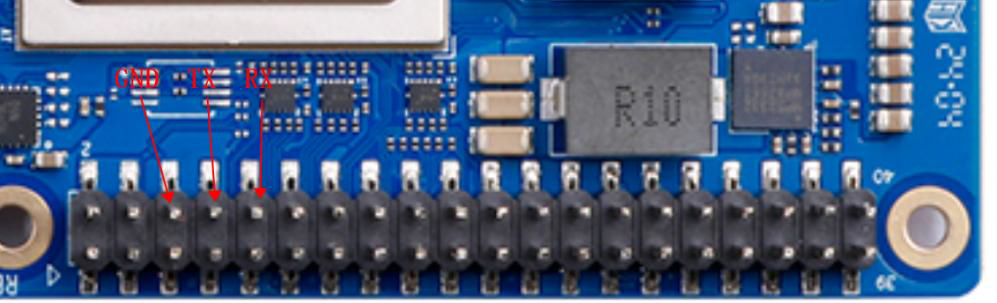
\includegraphics{img1/gpio_ttl.png},开发板的TX(GPIO8)接入USB2TTL模块的RX接口,开发板的RX(GPIO10)则接入模块的TX接口,并连接好GND接地,在Windows电脑下可以使用PUTTY连接串口。
\item
  使用开发板自带的Micro
  USB接口进行串口调试,该方法更为方便,只需要一根Micro
  USB数据线,接入电脑后打开设备管理器查询对应的串口,然后使用PUTTY进行链接即可。
  以Micro USB接口为例:
\item
  使用Micro USB数据线连接开发板和电脑
\item
  打开电脑的设备管理器,选择端口,寻找开发板对应的串口端口号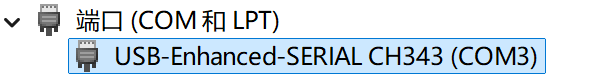
\includegraphics{img1/ttl.png}
\item
  打开串口调试软件(PUTTY)\includegraphics{img1/putty.png},将Connection
  Type选择为\texttt{Serial},然后在Serial
  Line处将端口号修改为设备管理器中查到的端口号,如作者此处端口号为\texttt{COM3},此外,还需要将Speed从9600修改为115200,最后点击Open打开串口。
\item
  等待出现\texttt{Ubuntu\ 22.04.3\ LTS\ orangepiaipro\ ttyAM0}字样,输入登录的用户名HwHiAiUser并回车,然后输入密码Mind@123并回车,注意在输入密码的时候屏幕并不会显示任何东西,登陆后的界面如图所示。
  \includegraphics{img1/serial.png} \includegraphics{img1/login.png}
\end{enumerate}

\hypertarget{ubuntu-xfceux684cux9762ux4f7fux7528ux8bf4ux660e}{%
\subsection{Ubuntu
Xfce桌面使用说明}\label{ubuntu-xfceux684cux9762ux4f7fux7528ux8bf4ux660e}}

目前系统仅支持Ubuntu 22.04 - Jammy系统,内核版本为Linux 5.10 \#\#\#\#
当前版本适配情况
请详见香橙派官方的用户手册,有部分功能仅支持使用官方程序进行测试,无法直接从系统中调用,在使用过程中需注意这些限制。

\hypertarget{hdmiux53e3ux4f7fux7528}{%
\subsubsection{HDMI口使用}\label{hdmiux53e3ux4f7fux7528}}

开发板有两个HDMI2.0 接口,目前只有HDMI0 支持显示Linux
系统的桌面,当Linux 系统的桌面系统关闭时,HDMI0 和HDMI1 还可以用于NVR
二次开 发场景输出图片。

\hypertarget{ux97f3ux9891ux4f7fux7528}{%
\subsubsection{音频使用}\label{ux97f3ux9891ux4f7fux7528}}

Linux 内核没有适配耳机和HDMI 等的ALSA 音频驱动,此部分驱动还在开
发中,目前只能通过音频样例代码来测试耳机、HDMI 的音频播放和板载MIC
的录音功能。或者自行购买Linux系统免驱的USB外置声卡,经测试可以正常使用。


% 第二章
\chapter{昇腾310B边缘计算实战}
\section{章节总览}\label{ux7ae0ux8282ux603bux89c8}

本章系统阐述 Ascend CANN 软件栈的分层结构、模型从框架格式到 OM
的转换原理、转换工具 ATC 的关键参数、OM 文件组织结构、AscendCL (ACL)
推理编程模型、精度与性能验证方法以及工程级质量保障流水线建设。阅读完成后应满足:
1. 能解释 Driver / Runtime / Compiler / Toolkit / ACL
各组件职责及交互边界。 2. 能为任意主流视觉模型编写一份无二义性的 ATC
转换命令并说明参数意义。 3. 能通过脚本解析 OM
模型的输入输出信息、算子统计与内存占用估算。 4. 能以 C 或 Python
写出健壮的最小推理程序(含异常处理与资源释放)。 5.
能定位转换/推理常见错误,给出复现、分析与修复路径。 6. 能构建``转换 →
精度对齐 → 性能基线 → 回归监测''的自动流水线。

\section{CANN
软件栈分层与数据流}\label{cann-ux8f6fux4ef6ux6808ux5206ux5c42ux4e0eux6570ux636eux6d41}

\begin{longtable}[]{@{}
  >{\raggedright\arraybackslash}p{(\linewidth - 6\tabcolsep) * \real{0.1667}}
  >{\raggedright\arraybackslash}p{(\linewidth - 6\tabcolsep) * \real{0.1667}}
  >{\raggedright\arraybackslash}p{(\linewidth - 6\tabcolsep) * \real{0.3333}}
  >{\raggedright\arraybackslash}p{(\linewidth - 6\tabcolsep) * \real{0.3333}}@{}}
\toprule\noalign{}
\begin{minipage}[b]{\linewidth}\raggedright
层级
\end{minipage} & \begin{minipage}[b]{\linewidth}\raggedright
组件
\end{minipage} & \begin{minipage}[b]{\linewidth}\raggedright
核心职责
\end{minipage} & \begin{minipage}[b]{\linewidth}\raggedright
典型交互
\end{minipage} \\
\midrule\noalign{}
\endhead
\bottomrule\noalign{}
\endlastfoot
硬件抽象 & Driver & 设备初始化、资源枚举、功耗/温度接口 & npu-smi /
Runtime \\
运行时 & Runtime & 上下文(Context)管理、Stream/Task 调度、内存分配 & ACL
/ Compiler \\
编译优化 & Graph Compiler &
图解析、拓扑排序、算子匹配、内存复用、算子融合 & ATC / Runtime \\
工具链 & Toolkit & ATC 转换、Profiling、Dump、可视化、日志 & 开发者 \\
API 层 & AscendCL & C 接口封装:模型管理 / 内存 / 数据传输 / 执行 &
应用 \\
\end{longtable}

数据流(框架模型 → OM → 推理)核心阶段: 1. 前端导出:PyTorch →
ONNX(维度常量化、算子展开)。 2. ATC 编译:图解析 → Shape Infer →
算子选择 → Kernel 排布 → 内存映射 → 生成 OM(二进制 + 元数据段)。 3.
运行加载:aclmdlLoadFromFile 读取 OM Header,分配 Device
内存,构建执行计划(Task 列表)。 4. 推理执行:Host 侧准备输入 → H2D
拷贝 → Runtime 提交 Task → 硬件执行 → D2H 拷贝 → 后处理。

\section{环境一致性与安装验证}\label{ux73afux5883ux4e00ux81f4ux6027ux4e0eux5b89ux88c5ux9a8cux8bc1}

环境差异是隐性失败根源,建议形成``安装后自检''脚本,校验以下要点: 1.
版本矩阵:固件/Driver/CANN/ATC 必须在官方 Release Note 支持组合内。 2.
环境变量:\passthrough{\lstinline!ASCEND\_INSTALL\_PATH!}
指向安装根;\passthrough{\lstinline!LD\_LIBRARY\_PATH!} 中包含
\passthrough{\lstinline!driver!} 与
\passthrough{\lstinline!runtime/lib64!};Python 绑定需在
\passthrough{\lstinline!PYTHONPATH!} 中。 3.
设备可见:\passthrough{\lstinline!npu-smi info!} 返回芯片型号
\passthrough{\lstinline!Ascend310B!} 且状态正常,无
\passthrough{\lstinline!Fault!} 标记。 4.
转换工具:\passthrough{\lstinline!atc --version!}
输出版本与期望匹配;\passthrough{\lstinline!atc --help!}
能正常列出参数。 5. 运行权限:当前用户具备访问
\passthrough{\lstinline!/dev/davinci*!}
设备节点读写权限(若无,加入相应用户组或 udev 规则)。 6. Python
依赖:\passthrough{\lstinline!numpy!}, \passthrough{\lstinline!onnx!},
\passthrough{\lstinline!onnxruntime!} (精度对齐),
\passthrough{\lstinline!pyyaml!}, 自编写工具包。

\section{模型准备与输入规范统一}\label{ux6a21ux578bux51c6ux5907ux4e0eux8f93ux5165ux89c4ux8303ux7edfux4e00}

\begin{longtable}[]{@{}lll@{}}
\toprule\noalign{}
项 & 说明 & 决策标准 \\
\midrule\noalign{}
\endhead
\bottomrule\noalign{}
\endlastfoot
边界 Shape & 静态 or 动态 & 场景多尺寸/Batch 波动? \\
Layout & NCHW / NHWC & 上游预处理 \& 算子最佳实现 \\
颜色空间 & RGB / BGR / YUV & 原始采集格式 + 算子期望 \\
归一化 & mean/std / scale & 训练环节定义必须完全对齐 \\
精度策略 & FP16 / INT8 & 性能目标 \& 可接受精度损失 \\
Quant 校准集 & 代表性样本 & 覆盖亮度/场景/尺寸多样性 \\
\end{longtable}

核心风险:训练与部署输入不一致(尺寸拉伸方式、通道顺序、归一化顺序、色彩空间转换位置)。必须输出``输入契约文件''(JSON/YAML)标注:\passthrough{\lstinline!shape!}、\passthrough{\lstinline!dtype!}、\passthrough{\lstinline!layout!}、\passthrough{\lstinline!color\_space!}、\passthrough{\lstinline!mean/std!}、\passthrough{\lstinline!range!}、\passthrough{\lstinline!precision\_mode!}。

\section{ATC
模型转换详解}\label{atc-ux6a21ux578bux8f6cux6362ux8be6ux89e3}

典型命令(以 ResNet50 为例,支持 FP16):

\begin{lstlisting}
atc \
  --model=resnet50.onnx \
  --framework=5 \
  --output=resnet50_fp16 \
  --input_format=NCHW \
  --input_shape="input:1,3,224,224" \
  --soc_version=Ascend310B \
  --precision_mode=allow_fp32_to_fp16 \
  --op_select_implmode=high_performance \
  --log=info \
  --insert_op_conf=aipp.cfg
\end{lstlisting}

关键参数说明: \textbar{} 参数 \textbar{} 作用 \textbar{} 注意事项
\textbar{} \textbar{} ---- \textbar{} ---- \textbar{} --------
\textbar{} \textbar{} \passthrough{\lstinline!--framework!} \textbar{}
输入框架类型 (5=ONNX) \textbar{} 与实际导出一致,否则形状推理异常
\textbar{} \textbar{} \passthrough{\lstinline!--input\_shape!}
\textbar{} 静态 shape 指定 \textbar{} 多输入以逗号分隔
\passthrough{\lstinline!in1:1,3,224,224;in2:1,128!} \textbar{}
\textbar{} \passthrough{\lstinline!--dynamic\_batch\_size!} \textbar{}
动态 Batch \textbar{} 与 \passthrough{\lstinline!--input\_shape!}
不能混用静态冲突 \textbar{} \textbar{}
\passthrough{\lstinline!--dynamic\_image\_size!} \textbar{} 动态分辨率
\textbar{} YOLO 等多尺度部署 \textbar{} \textbar{}
\passthrough{\lstinline!--precision\_mode!} \textbar{} 精度策略
\textbar{}
\passthrough{\lstinline!allow\_mix\_precision!}、\passthrough{\lstinline!allow\_fp32\_to\_fp16!}
\textbar{} \textbar{} \passthrough{\lstinline!--soc\_version!}
\textbar{} 硬件目标 \textbar{} 与实际芯片匹配;310B 与 310P 不可混淆
\textbar{} \textbar{} \passthrough{\lstinline!--insert\_op\_conf!}
\textbar{} AIPP(预处理) \textbar{} 可下沉色彩空间转换、均值/方差
\textbar{} \textbar{} \passthrough{\lstinline!--op\_select\_implmode!}
\textbar{} 算子实现优先级 \textbar{}
\passthrough{\lstinline!high\_precision!} vs
\passthrough{\lstinline!high\_performance!} \textbar{} \textbar{}
\passthrough{\lstinline!--input\_format!} \textbar{} 模型输入排布
\textbar{} 与 \passthrough{\lstinline!--input\_shape!} 一致性检查
\textbar{} \textbar{} \passthrough{\lstinline!--output\_type!}
\textbar{} 输出 dtype \textbar{} 常用于 INT8 推理后转 FP32 便于后处理
\textbar{} \textbar{} \passthrough{\lstinline!--enable\_small\_channel!}
\textbar{} 小通道优化 \textbar{} 某些轻量网络加速 \textbar{}

\subsection{自定义算子加载}\label{ux81eaux5b9aux4e49ux7b97ux5b50ux52a0ux8f7d}

\begin{enumerate}
\def\labelenumi{\arabic{enumi}.}
\tightlist
\item
  定义 JSON 描述(输入输出、属性)。
\item
  编写 Kernel 源码并使用官方编译脚本生成 \passthrough{\lstinline!.so!}。
\item
  ATC 阶段通过 \passthrough{\lstinline!--optypelist\_for\_impl!} 或
  \passthrough{\lstinline!--soc\_version!} + JSON 注册;运行时放置在
  \passthrough{\lstinline!ASCEND\_OPP\_PATH!} 对应目录。
\end{enumerate}

\subsection{日志与告警}\label{ux65e5ux5fd7ux4e0eux544aux8b66}

常见告警分类: - 未使用节点 (prune) → 确认是否为训练辅助算子 (e.g.,
Dropout)。 - 算子降级 → 检查是否 fallback 到
Host;对性能敏感需重写/替换结构。 - 精度截断 →
记录发生算子,评估对最终指标影响;必要时关闭相关优化策略。

\section{OM 文件结构解读}\label{om-ux6587ux4ef6ux7ed3ux6784ux89e3ux8bfb}

OM 通常包含: 1. Header:魔数、版本、输入输出 Tensor
数、DataType、Format。 2. Graph
Meta:节点拓扑、算子类型列表、权重偏移指针。 3. Weights
Segment:连续存放常量权重与常量张量。 4. Task List:调度指令列表(Kernel
Launch / MemCopy / Event)。 5. AIPP 配置(可选):预处理算子参数表。

\subsection{解析与统计脚本要点}\label{ux89e3ux6790ux4e0eux7edfux8ba1ux811aux672cux8981ux70b9}

\begin{itemize}
\tightlist
\item
  调用 \passthrough{\lstinline!aclmdlQuerySize!}
  得到模型工作内存与权重内存需求。
\item
  利用 \passthrough{\lstinline!aclmdlGetInputIndexByName!} /
  \passthrough{\lstinline!aclmdlGetInputDims!} 获取 IO 维度与 dtype。
\item
  自建表格:\passthrough{\lstinline!\{op\_type: count\}!}
  用于识别热点类型(后续优化参考)。
\end{itemize}

\section{ACL
推理编程模型}\label{acl-ux63a8ux7406ux7f16ux7a0bux6a21ux578b}

典型生命周期: 1. 初始化:\passthrough{\lstinline!aclInit!} →
\passthrough{\lstinline!aclrtSetDevice!} →
\passthrough{\lstinline!aclrtCreateContext!} → (可选) 创建 Stream。 2.
模型:\passthrough{\lstinline!aclmdlLoadFromFile!} → 查询 IO 描述 →
预分配 Device Buffer。 3. 数据准备:Host 侧申请内存(Pinned 优先)→
格式/归一化 → H2D 拷贝。 4.
执行:\passthrough{\lstinline!aclmdlExecute!} 或 异步
\passthrough{\lstinline!aclmdlExecuteAsync!} + Stream 同步。 5.
输出处理:D2H 拷贝 → 解码 / Softmax / NMS。 6.
资源释放:\passthrough{\lstinline!aclmdlUnload!} → Free buffers →
Destroy Context → \passthrough{\lstinline!aclFinalize!}。

\subsection{C
语言最小示例(核心片段)}\label{c-ux8bedux8a00ux6700ux5c0fux793aux4f8bux6838ux5fc3ux7247ux6bb5}

\begin{lstlisting}
// 省略错误检查宏定义 ERR_CHK
aclInit(NULL);
aclrtSetDevice(0);
aclrtContext ctx; aclrtCreateContext(&ctx, 0);
uint32_t modelId; size_t wSize, rSize;
aclmdlLoadFromFile("resnet50_fp16.om", &modelId);
aclmdlDesc *desc = aclmdlCreateDesc();
aclmdlGetDesc(desc, modelId);
// 输入准备
void *hostIn = malloc(3*224*224*2); // FP16
void *devIn; aclrtMalloc(&devIn, 3*224*224*2, ACL_MEM_MALLOC_NORMAL_ONLY);
aclrtMemcpy(devIn, 3*224*224*2, hostIn, 3*224*224*2, ACL_MEMCPY_HOST_TO_DEVICE);
aclmdlDataset *input = aclmdlCreateDataset();
aclDataBuffer *inBuf = aclCreateDataBuffer(devIn, 3*224*224*2);
aclmdlAddDatasetBuffer(input, inBuf);
// 输出
size_t outSize = 1000 * 2; // FP16 logits
void *devOut; aclrtMalloc(&devOut, outSize, ACL_MEM_MALLOC_NORMAL_ONLY);
aclmdlDataset *output = aclmdlCreateDataset();
aclDataBuffer *outBuf = aclCreateDataBuffer(devOut, outSize);
aclmdlAddDatasetBuffer(output, outBuf);
aclmdlExecute(modelId, input, output);
// 回拷
void *hostOut = malloc(outSize);
aclrtMemcpy(hostOut, outSize, devOut, outSize, ACL_MEMCPY_DEVICE_TO_HOST);
// 解析 softmax ...
// 清理省略
\end{lstlisting}

\subsection{Python 封装思路}\label{python-ux5c01ux88c5ux601dux8def}

官方 Python 包接口层次相似,建议封装
\passthrough{\lstinline!ModelSession!} 类:

\begin{lstlisting}
class ModelSession:
    def __init__(self, om_path):
        self.model_id = load(om_path)
        self.desc = query(self.model_id)
        self._alloc_io_buffers()
    def infer(self, np_input: np.ndarray):
        # preprocess -> copy H2D -> execute -> copy D2H -> postprocess
        return logits
    def __del__(self):
        self._release()
\end{lstlisting}

\section{性能与初步调优策略}\label{ux6027ux80fdux4e0eux521dux6b65ux8c03ux4f18ux7b56ux7565}

\begin{longtable}[]{@{}llll@{}}
\toprule\noalign{}
问题 & 诊断信号 & 初级优化 & 进阶优化 \\
\midrule\noalign{}
\endhead
\bottomrule\noalign{}
\endlastfoot
时延波动大 & P95 \textgreater\textgreater{} P50 & 固定 Batch / 预热 &
Stream 并行 + Pin 内存 \\
吞吐不足 & 利用率低 & FP16 & 多实例并行 \\
拷贝过多 & H2D 大占比 & 合并预处理 & AIPP 下沉 \\
算子退化 & 日志 Fallback & 替换模型结构 & 自定义算子 \\
\end{longtable}

关键早期收集指标:平均时延、P95、H2D+Pre
占比、推理核心阶段占比、内存峰值。

\section{常见错误分类与排查路径}\label{ux5e38ux89c1ux9519ux8befux5206ux7c7bux4e0eux6392ux67e5ux8defux5f84}

\begin{longtable}[]{@{}
  >{\raggedright\arraybackslash}p{(\linewidth - 8\tabcolsep) * \real{0.1250}}
  >{\raggedright\arraybackslash}p{(\linewidth - 8\tabcolsep) * \real{0.2500}}
  >{\raggedright\arraybackslash}p{(\linewidth - 8\tabcolsep) * \real{0.2500}}
  >{\raggedright\arraybackslash}p{(\linewidth - 8\tabcolsep) * \real{0.2500}}
  >{\raggedright\arraybackslash}p{(\linewidth - 8\tabcolsep) * \real{0.1250}}@{}}
\toprule\noalign{}
\begin{minipage}[b]{\linewidth}\raggedright
场景
\end{minipage} & \begin{minipage}[b]{\linewidth}\raggedright
日志/现象
\end{minipage} & \begin{minipage}[b]{\linewidth}\raggedright
根因类型
\end{minipage} & \begin{minipage}[b]{\linewidth}\raggedright
排查步骤
\end{minipage} & \begin{minipage}[b]{\linewidth}\raggedright
修复
\end{minipage} \\
\midrule\noalign{}
\endhead
\bottomrule\noalign{}
\endlastfoot
ATC Unsupported Op & E190xx & 模型含新算子 & onnxsim → 拆解 &
替换/重写 \\
动态 Shape OOM & 执行时内存溢出 & 最大分辨率超预算 & 统计输入分布 &
分桶/裁剪 \\
精度下降 & Top1 -5\% & 归一化差异 & 离线对齐脚本 & 修正预处理 \\
输出 NAN & logits 异常 & 上溢/量化尺度错误 & Dump 中间 Tensor &
重新校准 \\
设备不可见 & aclInit 失败 & Driver 未加载 & dmesg \& npu-smi &
重装驱动 \\
\end{longtable}

\section{质量保障与自动化流水线}\label{ux8d28ux91cfux4fddux969cux4e0eux81eaux52a8ux5316ux6d41ux6c34ux7ebf}

流水线阶段: 1. Export:框架导出 + ONNX Simplify +
模型签名(\passthrough{\lstinline!inputs/name/dtype/layout/mean/std!}).
2. Convert:ATC 命令模板参数化(YAML → 渲染)。 3. Validate:ONNXRuntime
vs OM 输出差异 (L1/L2/TopK 差异率 \textless{} 阈值)。 4.
Benchmark:Warmup N + Run M,记录 JSON
\passthrough{\lstinline!\{avg, p50, p95, memory\}!}。 5.
Archive:产物归档(om, atc.log, metrics.json, signature.json)。 6.
Regression:新提交对比基线差异,超阈值报警。

\subsection{精度对齐示例指标}\label{ux7cbeux5ea6ux5bf9ux9f50ux793aux4f8bux6307ux6807}

\begin{longtable}[]{@{}lll@{}}
\toprule\noalign{}
指标 & 计算方式 & 推荐阈值 \\
\midrule\noalign{}
\endhead
\bottomrule\noalign{}
\endlastfoot
Top1 差异 & abs(top1\_acc\_onnx - top1\_acc\_om) & ≤0.2\% \\
平均 L1 & mean( & y\_onnx - y\_om \\
最大相对误差 & max( & d \\
\end{longtable}

\section{Dump / Profiling /
调试手段}\label{dump-profiling-ux8c03ux8bd5ux624bux6bb5}

\begin{longtable}[]{@{}llll@{}}
\toprule\noalign{}
工具 & 使用时机 & 价值 & 代价 \\
\midrule\noalign{}
\endhead
\bottomrule\noalign{}
\endlastfoot
Dump 中间 Tensor & 精度异常 & 对齐中间层 & I/O 与存储占用 \\
Profiling Timeline & 性能不达标 & 定位瓶颈 & 额外开销 (W\%) \\
日志级别升高 (\passthrough{\lstinline!--log=debug!}) & 转换失败 &
细粒度错误码 & 噪声多 \\
校准数据捕获 & INT8 偏差大 & 重新校准 & 需准备代表性样本 \\
\end{longtable}

Dump 配置:通过环境变量或 JSON 指定层名称白名单,避免全量 Dump
导致性能与空间压力。

\section{动态 Shape
策略与内存规划}\label{ux52a8ux6001-shape-ux7b56ux7565ux4e0eux5185ux5b58ux89c4ux5212}

多分辨率/Batch 场景建议: 1. 分桶:统计历史尺寸 → 选 3\textasciitilde5
个``代表桶'' → ATC 生成多 OM;运行时按最近桶选择。 2. Padding:对齐到
32/64 边界,减少算子内部分支;记录真实尺寸用于后处理。 3.
内存预估:最大桶内存 + 安全冗余 15\% 作为部署阈值,超出触发降级。

\section{精度验证流程与脚本要点}\label{ux7cbeux5ea6ux9a8cux8bc1ux6d41ux7a0bux4e0eux811aux672cux8981ux70b9}

流程:采样输入集(校准集或验证集子集)→ ONNXRuntime 前向 → Ascend 前向 →
指标聚合 → 报告。 脚本关键: 1. 随机种子固定; 2.
输入预处理完全共用函数; 3. 支持逐层 Dump 比对(差异 \textgreater{} 阈值
输出层名)。

\section{安全与合规考量}\label{ux5b89ux5168ux4e0eux5408ux89c4ux8003ux91cf}

\begin{itemize}
\tightlist
\item
  模型资产:带版权或敏感权重需加密存储(考虑文件系统权限+传输校验
  hash)。
\item
  日志脱敏:避免输出用户数据路径/片段;开关化控制。
\item
  Dump
  数据:限定开发模式,生产禁用;数据自动过期删除策略(时间或数量)。
\end{itemize}

\section{章节小结}\label{ux7ae0ux8282ux5c0fux7ed3}

本章从宏观分层、转换编译、OM 结构、ACL
编程、性能与精度保障、调试工具、自动化流水线到动态 Shape
与安全实践建立了闭环。掌握这些内容后即可进入后续``边缘系统架构与部署实践''章节,扩展到多模型、多进程及系统级优化。

\section{实践任务}\label{ux5b9eux8df5ux4efbux52a1}

\begin{enumerate}
\def\labelenumi{\arabic{enumi}.}
\tightlist
\item
  任选一个公开 ONNX 分类模型(如 ResNet50)完成 ATC 转换,提交:命令 +
  atc.log。
\item
  以 C 或 Python 实现最小推理程序,输出前 5 TopK 结果与 softmax 概率。
\item
  编写对齐脚本比较 50 张图片 ONNX vs OM 输出差异(报告 L1/Top1 差异)。
\item
  收集 Profiling Timeline,列出前 3 耗时算子类型及优化建议。
\item
  输出
  \passthrough{\lstinline!signature.json!}、\passthrough{\lstinline!metrics.json!}、\passthrough{\lstinline!conversion\_meta.yaml!}
  并归档。
\end{enumerate}


% \chapter{引言}
% 昇腾310B实战——从入门到精通边缘计算

% \section{第一节}

% 这是一段示例文本,使用思源宋体显示。XeLaTeX 结合开源中文字体可以产生高质量的中文排版效果。\textbf{这是粗体文字},\textit{这是斜体文字}。

% \subsection{小节}

% 数学公式示例:爱因斯坦的质能方程 $E = mc^2$,以及行内公式 $\int_a^b f(x) dx$。

% 多行公式示例:
% \begin{equation}
% \frac{\partial u}{\partial t} = \alpha \nabla^2 u
% \end{equation}

% \section{第二节}

% \subsection{列表环境}

% 无序列表示例:
% \begin{itemize}
% \item 第一项
% \item 第二项
% \item 第三项
% \end{itemize}

% 有序列表示例:
% \begin{enumerate}
% \item 第一项
% \item 第二项
% \item 第三项
% \end{enumerate}

% \subsection{表格环境}

% 表格示例:
% \begin{table}[htbp]
% \centering
% \caption{示例表格}
% \begin{tabular}{|c|c|c|}
% \hline
% 姓名 & 年龄 & 职业 \\
% \hline
% 张三 & 25 & 工程师 \\
% 李四 & 30 & 教师 \\
% 王五 & 28 & 医生 \\
% \hline
% \end{tabular}
% \end{table}

% % 第二章
% \chapter{主要内容}

% \section{定理环境示例}

% \begin{definition}[可微函数]
% 设函数 $f: U \subseteq \mathbb{R}^n \to \mathbb{R}$,如果存在线性映射 $A: \mathbb{R}^n \to \mathbb{R}$ 使得
% \[
% f(x + h) = f(x) + A(h) + o(\|h\|)
% \]
% 则称 $f$ 在点 $x$ 处可微。
% \end{definition}

% \begin{theorem}[中值定理]
% 如果函数 $f(x)$ 在闭区间 $[a, b]$ 上连续,在开区间 $(a, b)$ 内可导,则存在一点 $c \in (a, b)$ 使得
% \[
% f'(c) = \frac{f(b) - f(a)}{b - a}
% \]
% \end{theorem}

% \begin{proof}
% 这是定理的证明过程。可以使用罗尔定理来证明中值定理。
% \end{proof}

% \begin{example}
% 这是一个例子环境,用于展示示例内容。
% \end{example}

% % 参考文献
% \backmatter
% \chapter{参考文献}

% \nocite{*} % 显示所有参考文献,即使未被引用
% \bibliographystyle{plain} % 参考文献样式
% \bibliography{references} % 参考文献数据库

% % 附录
% \appendix
% \chapter{附录标题}

% 这里是附录内容。

\end{document}